\documentclass[a4paper]{report}
\usepackage[utf8]{inputenc}
\usepackage[T1]{fontenc}
\usepackage[french]{babel}

%============================================================

\usepackage{minted}
\usepackage{graphicx}
\usepackage[dvipsnames]{xcolor}
\usepackage[bookmarks]{hyperref}

%============================================================

\usepackage[style=numeric, sorting=ynt, natbib=true]{biblatex}
\addbibresource{rapport.bib}

%============================================================

\usepackage{array}
\usepackage{xspace}
\usepackage{tabularx}

\usepackage{enumitem}
\setlist[itemize]{leftmargin=*}

\usepackage{caption}
\DeclareCaptionFormat{empty}{#1}
\renewcommand*\figurename{}

\makeatletter
\renewcommand\verbatim@font{\normalfont\fontencoding{T1}\ttfamily}
\makeatother

%============================================================

\usepackage{amsmath}  % align*
\usepackage{amssymb}  % mathbb
\usepackage{mathrsfs} % mathscr
\usepackage{scalerel} % scalerel
\usepackage{mathtools}  % mathclap

%============================================================

\usepackage{mathpartir}
\def\RightTirNameStyle{\textnormal}

%============================================================

\usepackage{amsthm}

\newtheoremstyle{definition}
  {}    % space above
  {}    % space below
  {}    % body font
  {}    % indent
  {\bf} % head font
  {\\}  % head punctuation
  { }   % head space
  {}    % head spec

\newenvironment{preuve} 
  {\begin{proof}~\\} 
  {\end{proof}}

\theoremstyle{definition}

\newtheorem{theoreme}{Théorème}
\newtheorem{definition}[theoreme]{Définition}
\newtheorem{lemme}[theoreme]{Lemme}
\newtheorem{exemple}[theoreme]{Exemple}

\makeatletter
\@addtoreset{theoreme}{section}
\@addtoreset{theoreme}{subsection}
\@addtoreset{theoreme}{subsubsection}
\newcommand{\theoremeprefix}{}
\let\thetheoremesaved\thetheoreme
\renewcommand{\thetheoreme}{\theoremeprefix\thetheoremesaved}
\let\sectionsaved\section
\patchcmd{\@startsection}{\par}{\renewcommand{\theoremeprefix}{\csname the#1\endcsname.}}{}{}
\makeatother

%============================================================

\newcommand{\dowsindex}{\texttt{dowsindex}\xspace}

\newcommand{\interval}[2]{[\![#1\,;#2]\!]}
\newcommand{\mset}[1]{\{\![#1]\!\}}

\newcommand{\qeq}{\stackrel {\scriptscriptstyle ?} =}

\newcommand{\ssi}{\textit{ssi}\xspace}
\newcommand{\unit}{\bold{unit}}
\newcommand{\norm}{\mathrm{norm}}

\newcommand{\V}{\mathscr{V}}
\newcommand{\F}{\mathscr{F}}
\newcommand{\E}{\mathscr{E}}
\newcommand{\G}{\mathscr{G}}
\newcommand{\T}{\mathrm{T}}
\newcommand{\N}{\mathrm{N}}

\newcommand{\mathhyphen}{{\hbox{-}}}

\DeclareMathOperator*{\msetN_bigplus}{\scalerel*{+}{\sum}^\#_\N}
\DeclareMathOperator*{\msetG_bigplus}{\scalerel*{+}{\sum}^\#_\G}

%============================================================

\title{Recherche de fonctions \\ par \\ unification modulo isomorphismes de types}
\author{Clément ALLAIN \\ Stage de M1 encadré par Gabriel RADANNE}
\date{Juin 2021}

%============================================================

\begin{document}

\maketitle

\tableofcontents

\newpage

%============================================================
%============================================================
%============================================================

\chapter{Introduction}

S'il est une chose dont on a besoin en programmation fonctionnelle, c'est bien de fonctions. Seulement voilà, ce n'est pas si simple. Mettre la main sur l'une d'entre elles en présence d'un environnement de grande taille s'avère parfois difficile, à tout le moins fastidieux. Aussi, remédions.

Il s'agit de mettre sur pied un système de recherche de fonctions pour le langage OCaml \cite{OCaml}. L'écosystème en est principalement composé des paquets OPAM --- des centaines de milliers d'identificateurs. Un tel outil épargnerait à l'utilisateur la peine de fouiller telle ou telle bibliothèque dans l'espoir d'y trouver une fonction s'accordant à son usage.

Mais que chercher et comment ? Des travaux similaires ont été menés notamment par Rittri pour Lazy ML \cite{Rittri91, Rittri93} et Delahaye pour Coq \cite{Delahaye}. Nous empruntons à notre tour à Rittri \cite{Rittri91} le tableau \ref{tab_fold}.

\begin{table}[h]
  \centering
  \begin{tabular}{|l|l|l|}
    \hline
      Langage &
      Nom &
      Type
    \\
    \hline
      LCF ML \cite{LCF_ML} &
      \texttt{itlist} &
      $(\alpha \rightarrow \beta \rightarrow \beta) \rightarrow list (\alpha) \rightarrow \beta \rightarrow \beta$
    \\
      Caml Light \cite{Caml_Light} &
      \texttt{list\_it} &
      $(\alpha \rightarrow \beta \rightarrow \beta) \rightarrow list (\alpha) \rightarrow \beta \rightarrow \beta$
    \\
      Haskell \cite{Haskell} &
      \texttt{foldr} &
      $(\alpha \rightarrow \beta \rightarrow \alpha) \rightarrow \alpha \rightarrow list (\beta) \rightarrow \alpha$
    \\
      SML of New Jersey \cite{SML_New_Jersey} &
      \texttt{fold} &
      $(\alpha \times \beta \rightarrow \beta) \rightarrow list (\alpha) \rightarrow \beta \rightarrow \beta$
    \\
      Edinburgh SML \cite{Edinburgh_SML} &
      \texttt{fold\_right} &
      $(\alpha \times \beta \rightarrow \beta) \rightarrow \beta \rightarrow list (\alpha) \rightarrow \beta$
    \\
    \hline
  \end{tabular}
  \caption{\label{tab_fold} Variations sur \texttt{List.fold\_left} d'OCaml dans plusieurs dialectes de Core-ML \cite{Core_ML}.}
\end{table}

Plusieurs observations en émanent. Une recherche par identificateur en l'espèce — une fonction se comportant comme \texttt{List.fold\_left} en OCaml — se heurterait à la diversité des noms potentiels. De même, une recherche syntaxique sur les types s'accommoderait mal des variations en un sens équivalentes de la forme du type. Pourtant, toutes ces fonctions font essentiellement le même travail ; cette diversité est due à l'arbitraire de l'auteur de la fonction.

Que faire, alors ? Une recherche par spécification s'avérerait bien plus satisfaisante, mais pas forcément décidable. On peut retenir comme spécification grossière le type d'une fonction — « \textit{type as search key} » — tout en l'enrichissant par une approche sémantique et non plus purement syntaxique. La \textit{recherche modulo isomorphisme de type} s'est imposée dans la littérature. Elle consiste intuitivement à autoriser des réarrangements triviaux dans les types : permutations des paramètres et curryfication. Cette notion reste néanmoins à définir formellement, et surtout à décider algorithmiquement. Nous y consacrerons le chapitre 2.

Comme souligné par Rittri \cite{Rittri93}, il est bienvenu d'autoriser l'instantiation des types dans la recherche. Si la chose est seulement permise aux types issus de l'écosystème, il s'agit de \emph{matching} ; si le type demandé peut aussi être instancié, on parlera d'\emph{unification}. Gabriel Radanne a implémenté un algorithme d'unification présenté dans la dernière partie du chapitre 2.

Le système résultant ne saurait passer à l'échelle sans un travail sur les fonctions de l'écosystème préalable à la recherche. Dans le chapitre 3, nous proposerons une technique d'indexation reposant sur des conditions nécessaires d'unifiabilité. L'apport de cette technique se révélera substantiel.

Enfin, nous décrirons dans le chapitre 4 le fruit de notre travail : le programme \dowsindex.

%============================================================
%============================================================
%============================================================

\chapter{Unification modulo isomorphismes de types}

Nous éclairons dans ce chapitre la notion d'\emph{équivalence entre types} et la façon dont nous l'exploitons. Il s'agit de formaliser les réarrangements permis par des \emph{isomorphismes de types}. Intuitivement, deux types sont \emph{isomorphes} s'ils admettent deux fonctions de conversion permettant de passer de l'un à l'autre. L'\emph{unifiabilité modulo isomorphismes}, ajoute à cela la capacité d'instancier les types. Nous présentons également l'implémentation de Gabriel Radanne qui a servi de point de départ à ce stage.

%============================================================
%============================================================

\section{Définitions préliminaires}

Commençons par poser quelques définitions : \emph{types}, \emph{axiome équationnel}, \emph{théorie équationnelle}, \emph{unifiabilité}. Pour cela, on se donne un ensemble dénombrable $\V = \{ \alpha, \beta, \gamma, \delta, \dots \}$ de symboles de variables.

Le langage OCaml permet de définir de nouveaux types : types-sommes, enregistrements\ldots Nous aurons donc besoin de \emph{constructeurs de types}. Nous les formalisons par la notion de \emph{signature}.

\begin{definition}[signature]
  Une signature est un ensemble fini $\F$ de symboles de constructeurs muni d'une fonction d'arité $| \cdot |_\F$ de $\F$ dans $\mathbb{N}$ et tel que $\V \cap \F = \emptyset$. Les constructeurs d'arité nulle sont appelés constantes.
\end{definition}

\begin{exemple}
  Une signature $( \F, | \cdot |_\F )$ pour OCaml serait telle que :
  \begin{itemize}
    \item $int \in \F$ avec $| int |_\F = 0$ ;
    \item $float \in \F$ avec $| float |_\F = 0$ ;
    \item $bool \in \F$ avec $| bool |_\F = 0$ ;
    \item $list \in \F$ avec $| list |_\F = 1$ ;
    \item $array \in \F$ avec $| array |_\F = 1$ ;
    \item \dots
  \end{itemize}
\end{exemple}

Soit une signature $( \F, | \cdot |_\F )$ avec $\F = \{ f, \dots \}$.

%============================================================

\subsection{Types}

Définissons alors les \emph{types}. Un \emph{type} est soit :
\begin{itemize}[nosep]
  \item une variable ;
  \item le type $\unit$ ;
  \item un type-produit ;
  \item une type-flèche ;
  \item construit avec un symbole de la signature.
\end{itemize}

\begin{definition}[type]
  L'ensemble des types, noté $\T$, est défini inductivement par :
  \begin{mathpar}
      \inferrule* 
        { }
        {\V \subseteq \T}
      \and
      \inferrule*
        { }
        {\unit \in \T}
      \\
      \inferrule*
        {\tau_1 \in \T \\ \tau_2 \in \T}
        {\tau_1 \times \tau_2 \in \T}
      \and
      \inferrule*
        {\tau_1 \in \T \\ \tau_2 \in \T}
        {\tau_1 \rightarrow \tau_2 \in \T}
      \and
      \inferrule*
        {f \in \F \\ \overline\tau \in \T^{|f|_\F}}
        {f (\overline\tau) \in \T}
  \end{mathpar}
\end{definition}

On s'autorisera à omettre les parenthèses pour les constantes de $\F$. De façon usuelle, ajoutons que $\cdot \times \cdot$ et $\cdot \rightarrow \cdot$ sont associatifs à droite avec $\cdot \times \cdot$ de précédence plus élevée.

\begin{exemple}
  Avec la signature OCaml de l'exemple précédent, on a les types :
  \begin{itemize}
    \item $\unit \rightarrow int \times float$ ;
    \item $int \rightarrow (int \rightarrow \alpha) \rightarrow array (\alpha)$ ;
    \item $(\alpha \rightarrow \beta \rightarrow \alpha) \rightarrow \alpha \rightarrow list (\beta) \rightarrow \alpha$.
  \end{itemize}
\end{exemple}

\begin{definition}[variables d'un type]
  L'ensemble des variables d'un type $\tau$, noté $\mathrm{vars} (\tau)$, est défini inductivement par :
  \begin{align*}
      \mathrm{vars} (\alpha) &=
      \{ \alpha \}
    \\
      \mathrm{vars} (\unit) &=
      \{ \}
    \\
      \mathrm{vars} (\tau_1 \times \tau_2) &=
      \mathrm{vars} (\tau_1) \cup \mathrm{vars} (\tau_2)
    \\
      \mathrm{vars} (\tau_1 \rightarrow \tau_2) &=
      \mathrm{vars} (\tau_1) \cup \mathrm{vars} (\tau_2)
    \\
      \mathrm{vars} (f (\overline\tau)) &=
      \bigcup_{i \in \interval 1 {|f|_\F}} \mathrm{vars} (\overline\tau_i)
  \end{align*}
\end{definition}

Dans la suite, il nous faudra \emph{instancier} un type : il s'agit de substituer une ou plusieurs variables par des types correspondants. Un type sera vu comme \emph{moins général} qu'un autre s'il est obtenu en substituant dans ce dernier.

\begin{definition}[substitution de types]
  Une substitution de types est une fonction de $\V$ dans $\T$. \\
  On note $\Sigma$ l'ensemble des substitution de types.
\end{definition}

\begin{definition}[domaine d'une substitution de types]
  Le domaine d'une substitution de types $\sigma$, noté $\mathrm{dom} (\sigma)$, est l'ensemble :
  \[ \{ \alpha \in \V \mid \hat\sigma (\alpha) \neq \alpha \} \]
\end{definition}

Lorsque le domaine d'une substitution $\sigma$ est fini de cardinal $n$ — disons $\mathrm{dom} (\sigma) = \{ \alpha_1, \dots, \alpha_n \}$ —, on s'autorisera à la noter $\{ \alpha_1 \mapsto \sigma (\alpha_1), \dots, \alpha_n \mapsto \sigma (\alpha_n) \}$.

\begin{definition}[extension d'une substitution de types]
  L'extension d'une substitution de types $\sigma$, notée $\hat\sigma$, est l'unique endomorphisme de $\T$ dont la restriction à $\V$ est $\sigma$. \\
  Autrement dit, $\hat\sigma$ est définie inductivement par :
  \begin{align*}
      \hat\sigma (\alpha) &=
      \sigma (\alpha)
    \\
      \hat\sigma (\unit) &=
      \unit
    \\
      \hat\sigma (\tau_1 \times \tau_2) &=
      \hat\sigma (\tau_1) \times \hat\sigma (\tau_2)
    \\
      \hat\sigma (\tau_1 \rightarrow \tau_2) &=
      \hat\sigma (\tau_1) \rightarrow \hat\sigma (\tau_2)
    \\
      \hat\sigma (f (\tau_1, \dots, \tau_{|f|_\F})) &=
      f (\hat\sigma (\tau_1), \dots, \hat\sigma (\tau_{|f|_\F}))
  \end{align*}
\end{definition}

\begin{definition}[$\leqslant_\Sigma$]
  Une substitution $\sigma_1$ est plus générale qu'une substitution $\sigma_2$, noté $\sigma_1 \leqslant_\Sigma \sigma_2$, \ssi il existe une substitution $\sigma_1'$ telle que $\sigma_2 = \sigma_1' \circ \sigma_1$.
\end{definition}

\begin{definition}[instance de type]
  Un type $\tau_1$ est une instance d'un type $\tau_2$, noté $\tau_2 \leqslant_\T \tau_1$, \ssi il existe une substitution $\sigma$ telle que $\tau_1 = \hat\sigma (\tau_2)$.
\end{definition}

\begin{exemple}
  Toujours avec la signature OCaml, on a les instances :
  \begin{itemize}
    \item $int \times int \leqslant_\T int \times int$ ;
    \item $\alpha \rightarrow \beta \leqslant_T \beta \rightarrow \alpha \leqslant_\T \alpha \rightarrow \beta$ ;
    \item $\alpha \rightarrow list (alpha) \rightarrow \unit \leqslant_\T int \rightarrow list (int) \rightarrow \unit$.
  \end{itemize}
\end{exemple}

%============================================================

\subsection{Théorie équationnelle}

Passées ces premières définitions, nous savons de qui nous parlons. Abordons maintenant la notion de \emph{théorie équationnelle}. Le plus important est la donnée des \emph{axiomes équationnels}, qui exprimeront les \emph{isomorphismes de types} qui nous intéressent et feront toute la force et la difficulté de l'\emph{unification modulo isomorphismes}. En découle naturellement une \emph{théorie équationnelle} : la plus petite congruence contenant les instances des axiomes.

\begin{definition}[axiome équationnel]
  Un axiome équationnel est un couple de types de la forme $\tau_1 \cong_\T \tau_2$.
\end{definition}

\begin{definition}[système équationnel]
  Un système équationnel est un ensemble d'axiomes équationnels.
\end{definition}

\begin{definition}[instance d'axiome équationnel]
  Une instance d'un axiome équationnel $\tau_1 \cong_\T \tau_2$ est un couple de types $(\tau_1', \tau_2')$ tel que $\tau_1 \leqslant_\T \tau_1'$ et $\tau_2 \leqslant_\T \tau_2'$.
\end{definition}

\begin{definition}[théorie équationnelle, $\E$-équivalence]
  Soit un système équationnel $\E$. \\
  La théorie équationnelle induite par $\E$, notée $\cdot \equiv_\T^\E \cdot$, est la plus petite congruence par rapport à $\F$ sur les types contenant toutes les instances des axiomes équationnels de $\E$. \\
  Autrement dit, c'est la plus petite relation binaire satisfaisant les règles d'inférence :
  \begin{mathpar}
    \inferrule*
      [right = ($\equiv_\T^\E$-ax)]
      {\tau_1 \cong_\T \tau_2 \in \E}
      {\hat\sigma (\tau_1) \equiv_\T^\E \hat\sigma (\tau_2)}
    \and
    \inferrule*
      [right = ($\equiv_\T^\E$-refl)]
      { }
      {\tau \equiv_\T^\E \tau}
    \\
    \inferrule*
      [right = ($\equiv_\T^\E$-trans)]
      {\tau_1 \equiv_\T^\E \tau_2 \\ \tau_2 \equiv_\T^\E \tau_3}
      {\tau_1 \equiv_\T^\E \tau_3}
    \and
    \inferrule*
      [right = ($\equiv_\T^\E$-sym)]
      {\tau_1 \equiv_\T^\E \tau_2}
      {\tau_2 \equiv_\T^\E \tau_1}
    \\
    \inferrule*
      [right = ($\equiv_\T^\E$-$\times_1$)]
      {\tau_1 \equiv_\T^\E \tau_1'}
      {\tau_1 \times \tau_2 \equiv_\T^\E \tau_1' \times \tau_2}
    \and
    \inferrule*
      [right = ($\equiv_\T^\E$-$\times_2$)]
      {\tau_2 \equiv_\T^\E \tau_2'}
      {\tau_1 \times \tau_2 \equiv_\T^\E \tau_1 \times \tau_2'}
    \\
    \inferrule*
      [right = ($\equiv_\T^\E$-$\rightarrow_1$)]
      {\tau_1 \equiv_\T^\E \tau_1'}
      {\tau_1 \rightarrow \tau_2 \equiv_\T^\E \tau_1' \rightarrow \tau_2}
    \and
    \inferrule*
      [right = ($\equiv_\T^\E$-$\rightarrow_2$)]
      {\tau_2 \equiv_\T^\E \tau_2'}
      {\tau_1 \rightarrow \tau_2 \equiv_\T^\E \tau_1 \rightarrow \tau_2'}
    \\
    \inferrule*
      [right = ($\equiv_\T^\E$-$\F$)]
      {f \in \F \\ i \in \interval 1 {|f|_\F} \\ \tau_i \equiv_\T^\E \tau_i'}
      {f (\tau_1, \dots, \tau_i, \dots, \tau_{|f|_\F}) \equiv_\T^\E f (\tau_1, \dots, \tau_i', \dots, \tau_{|f|_\F})}
  \end{mathpar}
  Si $\tau_1 \equiv_\T^\E \tau_2$, on dit que $\tau_1$ et $\tau_2$ sont $\E$-équivalents.
\end{definition}

\begin{exemple}
  Prenons comme axiomes $\E$ la commutativité et l'associativité du produit :
  \begin{align}
      \alpha \times \beta &\cong_\T
      \beta \times \alpha
      \tag{$\times$-comm}
    \\
      \alpha \times (\beta \times \gamma) &\cong_\T
      (\alpha \times \beta) \times \gamma
      \tag{$\times$-assoc}
  \end{align}
  En OCaml, les équivalences suivantes sont alors correctes :
  \begin{itemize}
    \item $\alpha \times int \rightarrow \beta \equiv_\T^\E int \times \alpha \rightarrow \beta$ ;
    \item $int \times float \times bool \times \unit \equiv_\T^\E float \times \unit \times int \times bool$.
  \end{itemize}
  En revanche, celles-ci ne le sont pas :
  \begin{itemize}
    \item $\alpha \times \beta \rightarrow \gamma \equiv_\T^\E \alpha \rightarrow \beta \rightarrow \gamma$ ;
    \item $\alpha \rightarrow (\beta \times \gamma) \equiv_\T^\E (\alpha \rightarrow \beta) \times (\alpha \rightarrow \gamma)$.
  \end{itemize}
\end{exemple}

Bien que la définition d'une théorie équationnelle ne mentionne pas la stabilité par substitution, c'en est un corollaire :

\begin{lemme}
  Si deux types $\tau_1$ et $\tau_2$ sont $\E$-équivalents, alors pour toute substitution $\sigma$, $\hat\sigma (\tau_1)$ et $\hat\sigma (\tau_2)$ sont $\E$-équivalents.
\end{lemme}

\begin{preuve}
  La preuve se fait par induction structurelle sur la dérivation de $\tau_1 \equiv_\T^\E \tau_2$ et par cas sur la dernière règle utilisée. Dans le cas ($\equiv_\T^\E$-ax), il s'agit de montrer que $\hat\sigma (\hat\sigma' (\tau_1))$ et $\hat\sigma (\hat\sigma' (\tau_2))$ sont $\E$-équivalents, où $\tau_1 \cong_\T \tau_2$ est un axiome de $\E$. Il suffit de remarquer que $\hat\sigma \circ \hat\sigma'$ est l'extension de la substitution $\hat\sigma \circ \sigma'$. Les autres cas sont triviaux.
\end{preuve}

%============================================================

\subsection{Matching et unification}

Nous en arrivons enfin aux notions fondamentales de \emph{matching} et \emph{unification}. Un type sujet \emph{matche} un type motif si l'on peut les rendre équivalents en instanciant le motif. Deux types sont \emph{unifiables} si l'on peut les rendre équivalents en les instanciant simultanément. En fait, on peut réduire le \emph{matching} à l'\emph{unification} en substituant chaque variable du sujet par une constante n'apparaissant pas dans le motif (de manière exclusive).

Soit un système équationnel $\E$.

\begin{definition}[$\E$-matcheur]
  Une substitution $\sigma$ est un $\E$-matcheur — ou encore matcheur modulo $\E$ — d'un type $\tau_1$ pour un type $\tau_2$ \ssi :
  \[ \tau_1 \equiv_\T^\E \hat\sigma (\tau_2) \]
\end{definition}

\begin{definition}[$\E$-matchabilité]
  Un type $\tau_1$ est $\E$-matchable — ou encore matchable modulo $\E$ — avec un type $\tau_2$ \ssi $\tau_1$ admet un $\E$-matcheur pour $\tau_2$.
\end{definition}

\begin{definition}[problème d'$\E$-matchabilité]
  Le problème d'$\E$-matchabilité — ou encore problème de matchabilité modulo $\E$ — consiste à déterminer si un type est matchable avec un autre.
\end{definition}

\begin{definition}[problème d'$\E$-matching]
  Soient $\tau_1$ et $\tau_2$ deux types. \\
  Le problème d'$\E$-matching — ou encore problème de matching modulo $\E$ — consiste à trouver un $\E$-matcheur de $\tau_1$ pour $\tau_2$.
\end{definition}

\begin{exemple}
  Reprenons le système équationnel $\E$ de l'exemple précédent. Les types OCaml suivants sont $\E$-matchables :
  \begin{itemize}
    \item $int \times \alpha \times float$ et $\beta \times \alpha$ avec $\{ \beta \mapsto int \times float \}$ ;
    \item $int \times float \rightarrow int$ et $\alpha \times \beta \rightarrow \beta$ avec $\{ \alpha \mapsto float, \beta \mapsto int \}$.
  \end{itemize}
\end{exemple}

\begin{definition}[$\E$-unificateur]
  Une substitution $\sigma$ est un $\E$-unificateur des types $\tau_1$ et $\tau_2$ \ssi :
  \[ \hat\sigma (\tau_1) \equiv_\T^\E \hat\sigma (\tau_2) \]
\end{definition}

\begin{definition}[$\E$-unifiabilité]
  Deux types $\tau_1$ et $\tau_2$ sont $\E$-unifiables — ou encore unifiables modulo $\E$ —, noté $\tau_1 \sim_\T^\E \tau_2$, \ssi ils admettent un $\E$-unificateur.
\end{definition}

\begin{definition}[problème d'$\E$-unifiabilité]
  Le problème d'$\E$-unifiabilité — ou encore problème d'unifiabilité modulo $\E$ — consiste à déterminer si deux types sont $\E$-unifiables.
\end{definition}

\begin{definition}[problème d'$\E$-unification]
  Soient $\tau_1$ et $\tau_2$ deux types. \\
  Le problème d'$\E$-unification — ou encore problème d'unification modulo $\E$ — consiste à trouver un $\E$-unificateur de $\tau_1$ et $\tau_2$.
\end{definition}

Lorsque $\E$ est vide, nous parlerons d'unification syntaxique ; dans le cas contraire, d'unification sémantique.

\begin{exemple}
  Avec le même système $\E$, les types OCaml suivants sont $\E$-unifiables :
  \begin{itemize}
    \item $int \times \alpha$ et $\beta \times float$ avec $\{ \alpha \mapsto float, \beta \mapsto int \}$ ;
    \item $\alpha \times \beta \rightarrow list (\alpha)$ et $list (\gamma) \times int \times float \rightarrow \gamma$ \\ avec $\{ \alpha \mapsto float \times int, \beta \mapsto list (\gamma), \gamma \mapsto list (\alpha) \}$.
  \end{itemize}
\end{exemple}

%============================================================
%============================================================

\section{Isomorphismes de types}

Ainsi parés, nous sommes à présent en mesure d'aborder le cœur de ce chapitre. Nous allons définir la notion d'équivalence entre types de notre système de recherche.

Les travaux de Mikael Rittri \cite{Rittri91, Rittri93} sur lesquels nous nous appuyons ont assis celle d'\emph{équivalence modulo isomorphismes de types}. La chose a fait l'objet de plusieurs recherches importantes, menées notamment par Giusseppe Longo, Kim Bruce, Roberto Di Cosmo \cite{Bruce_DiCosmo_Longo, DiCosmo92, DiCosmo93, DiCosmo95}, Sergei Soloviev \cite{Soloviev83, Soloviev93}, Paliath Narendran, Frank Pfenning et Richard Statman \cite{Narendran_Pfenning_Statman}.

%============================================================

\subsection{Isomorphismes de types en $\lambda$-calcul}

Dans cette section, on ignore les constructeurs de types : $\F$ est l'ensemble vide.

Les travaux cités auparavant décrivent les \emph{isomorphismes de types} dans plusieurs versions du $\lambda$-calcul simplement typé. Notons $\Lambda^1$ le $\lambda$-calcul simplement typé avec paires et élément terminal et $=_{\Lambda^1}$ l'égalité associée (pour plus de détails, voir par exemple \cite{DiCosmo95}). La notion d'\emph{isomorphisme de types} dans $\Lambda^1$ se définit ainsi :

\begin{definition}[isomorphisme de types dans $\Lambda^1$]
  Deux types $\tau_1$ et $\tau_2$ sont isomorphes dans $\Lambda^1$ \ssi il existe deux $\lambda$-termes $f : \tau_1 \rightarrow \tau_2$ et $g : \tau_2 \rightarrow \tau_1$ tels que $f \circ g =_{\Lambda^1} \mathrm{id}_{\tau_2}$ et $g \circ f =_{\Lambda^1} \mathrm{id}_{\tau_1}$.
\end{definition}

On peut donner une caractérisation équationnelle des isomorphismes de $\Lambda^1$. Ils correspondent aux isomorphismes valides dans les \emph{catégories cartésiennes fermées}. Longo, Bruce, Di Cosmo \cite{Bruce_DiCosmo_Longo} et Soloviev \cite{Soloviev83} ont démontré par deux méthodes différentes que les axiomes équationnels ci-dessous sont corrects et complets. On notera $\E^1$ la théorie équationnelle induite.
\begin{align}
    \alpha \times \beta &\cong_\T
    \beta \times \alpha
    \label{prod_comm}
    \tag{$\times$-comm}
  \\
    \alpha \times (\beta \times \gamma) &\cong_\T
    (\alpha \times \beta) \times \gamma
    \label{prod_assoc}
    \tag{$\times$-assoc}
  \\
    \unit \times \alpha &\cong_\T
    \alpha
    \label{prod_unit}
    \tag{$\times$-$\unit$}
  \\
    (\alpha \times \beta) \rightarrow \gamma &\cong_\T
    \alpha \rightarrow (\beta \rightarrow \gamma)
    \label{curry}
    \tag{curry}
  \\
    \unit \rightarrow \alpha &\cong_\T
    \alpha
    \label{curry_unit}
    \tag{curry-$\unit$}
  \\
    \alpha \rightarrow (\beta \times \gamma) &\cong_\T
    (\alpha \rightarrow \beta) \times (\alpha \rightarrow \gamma)
    \label{dist}
    \tag{dist}
  \\
    \alpha \rightarrow \unit &\cong_\T
    \unit
    \label{dist_unit}
    \tag{dist-$\unit$}
\end{align}

Néanmoins, Narendran, Pfenning et Statman \cite{Narendran_Pfenning_Statman} ont établi que, si le \emph{matching} modulo $\E^1$ est NP-complet, l'unification modulo $\E^1$ est indécidable. C'est ce qui a poussé Rittri \cite{Rittri93} à se concentrer sur les cinq premiers axiomes correspondant aux \emph{isomorphismes linéaires} (pour plus de détails, voir \cite{Rittri93}) complets dans les \emph{catégories monoïdales fermées symétriques} \cite{Soloviev93}. L'unification modulo cette nouvelle théorie est NP-complète \cite{Narendran_Pfenning_Statman}. Cet abandon des deux axiomes de distributivité \eqref{dist} et \eqref{dist_unit} — et donc de la complétude dans $\Lambda^1$ — s'avère d'après lui bénin, arguant que ces isomorphismes sont peu utiles en pratique.

%============================================================

\subsection{Isomorphismes de types en OCaml}

En outre, Di Cosmo \cite{DiCosmo92} a étudié les isomorphismes de types en Core-ML. De même, il en a tiré une axiomatisation équationnelle complète comportant de nouveaux isomorphismes. L'équivalence est alors décidable par un algorithme qu'il introduit dans \cite{DiCosmo95}. Malheureusement, cet algorithme ne s'adapte a priori pas directement au matching ou l'unification.

L'implémentation suit les préconisations de Rittri en renonçant à l'axiome \eqref{curry_unit}. En effet, bien qu'utile en pratique pour simuler une expression paresseuse, il complexifie l'algorithme d'unification. Ne s'agissant pas de l'isomorphisme le plus important, cela affecte peu la qualité de la recherche.

Reste donc les quatre premiers isomorphismes : \eqref{prod_comm}, \eqref{prod_assoc}, \eqref{prod_unit}, \eqref{curry}. Ils capturent exactement les réarrangements qui nous intéressent, en particulier la permutation des paramètres. Relevons toutefois que, si ces isomorphismes sont corrects pour Core-ML \cite{DiCosmo93}, leur correction pour OCaml n'est pas démontrée. Nous admettons ici qu'ils se « propagent » aux constructeurs de types, c'est-à-dire la congruence sur la signature OCaml.

Dans le reste de ce rapport, nous traiterons des types OCaml avec constructeurs. Nous dénoterons par $\E$ le système équationnel formé par les quatre axiomes, $\cdot \equiv_\T \cdot$ la théorie équationnelle induite par $\E$ et $\cdot \sim_\T \cdot$ l'$\E$-unifiabilité. Nous parlerons d'équivalence pour l'$\E$-équivalence, de matching pour l'$\E$-matching, d'unifiabilité pour l'$\E$-unifiabilité et d'unification pour l'$\E$-unification.

\begin{exemple}
  Les types suivants sont unifiables :
  \begin{itemize}
    \item $int \rightarrow float \rightarrow int \sim_\T float \rightarrow \alpha$ avec $\{ \alpha \mapsto int \rightarrow int \}$ ;
    \item $int \rightarrow \alpha \rightarrow \unit \sim_\T int \rightarrow \unit$ avec $\{ \alpha \mapsto \unit \}$ ;
    \item $int \rightarrow \alpha \rightarrow \unit \sim_\T int \rightarrow int \rightarrow int \rightarrow \unit$ avec $\{ \alpha \mapsto int \times int \}$ ;
    \item $(\alpha \rightarrow \beta \rightarrow \alpha) \rightarrow \alpha \rightarrow list (\beta) \rightarrow \alpha \sim_\T list (\gamma) \times \delta \rightarrow (\gamma \times \delta \rightarrow \delta) \rightarrow \delta$ \\ avec $\{ \gamma \mapsto \beta, \delta \mapsto \alpha \}$.
  \end{itemize}
\end{exemple}

%============================================================
%============================================================

\section{Implémentation de l'unification modulo isomorphismes}

%============================================================

\subsection{Algorithme d'unification syntaxique}

Avant d'aborder l'implémentation, revenons sur l'ancêtre commun des algorithmes d'unification sémantique, dû à Herbrand \cite{Herbrand}, Martelli et Montanari \cite{Martelli_Montanari}. Leur algorithme d'unification syntaxique consiste à transformer le problème initial par applications successives d'un certain nombre de règles afin d'aboutir à une forme résolue — essentiellement une substitution. La conception d'un algorithme d'unification sémantique repart souvent de ce principe, en modifiant les règles ou en en ajoutant.

Définissons tout d'abord les objets manipulés par l'algorithme : \emph{équations de types} et \emph{problèmes équationnels}.

\begin{definition}[équation de types]
  Une équation de types est un couple de types de la forme $\tau_1 \qeq \tau_2$.
\end{definition}

\begin{definition}[équation de types en forme résolue]
  Une équation de types est en forme résolue \ssi elle est de la forme $\alpha \qeq \tau$.
\end{definition}

\begin{definition}[problème équationnel]
  Un problème équationnel est un ensemble fini d'équations de types.
\end{definition}

\begin{definition}[problème en forme résolue]
  Un problème est en forme résolue \ssi il est de la forme :
  \[ \{ \alpha_1 \qeq \tau_1, \dots, \alpha_n \qeq \tau_n \} \]
  où chaque $\alpha_i$ n'apparaît qu'une seule fois. Il induit alors la substitution :
  \[ \{ \alpha_1 \mapsto \tau_1, \dots, \alpha_n \mapsto \tau_n \} \]
\end{definition}

On étend naturellement substitution, ensemble de variables et unificateur aux équations de types et problèmes équationnels.

Ceci étant fait, voyons maintenant comment \emph{transformer} un problème équationnel. Dans cette présentation, six règles suffisent :
\begin{itemize}
  \item (effacer) efface une équation triviale ;
  \item (orienter) réoriente une équation de la forme $\tau \qeq \alpha$, rendant (remplacer) potentiellement applicable ;
  \item (décomposer-$\times$), (décomposer-$\rightarrow$) et (décomposer-$\F$) décomposent respectivement un produit, une flèche et un type formé à l'aide d'un constructeur ;
  \item (substituer) substitue à l'aide d'une équation en forme résolue.
\end{itemize}

\begin{definition}[transformation d'un problème équationnel]
  Un problème équationnel $P_1$ se transforme en un problème $P_2$, noté $P_1 \rightsquigarrow P_2$, à l'aide les règles suivantes :
  \begin{mathpar}
    \inferrule*
      [right = (effacer)]
      {}
      {P \cup \{ \tau \qeq \tau \} \rightsquigarrow P}
    \\
    \inferrule*
      [right = (orienter)]
      {\tau \notin \V}
      {P \cup \{ \tau \qeq \alpha \} \rightsquigarrow P \cup \{ \alpha \qeq \tau \}}
    \\
    \inferrule*
      [right = (décomposer-$\times$)]
      {}
      {P \cup \{ \tau_1 \times \tau_2 \qeq \tau_1' \times \tau_2' \} \rightsquigarrow P \cup \{ \tau_1 \qeq \tau_1', \tau_2 \qeq \tau_2' \}}
    \\
    \inferrule*
      [right = (décomposer-$\rightarrow$)]
      {}
      {P \cup \{ \tau_1 \rightarrow \tau_2 \qeq \tau_1' \rightarrow \tau_2' \} \rightsquigarrow P \cup \{ \tau_1 \qeq \tau_1', \tau_2 \qeq \tau_2' \}}
    \\
    \inferrule*
      [right = (décomposer-$\F$)]
      {}
      {P \cup \{ f (\tau_1, \dots, \tau_{|f|_\F}) \qeq f (\tau_1', \dots, \tau_{|f|_\F}') \} \rightsquigarrow \\ P \cup \{ \tau_1 \qeq \tau_1', \dots, \tau_{|f|_\F} \qeq \tau_{|f|_\F}' \}}
    \\
    \inferrule*
      [right = (substituer)]
      {\alpha \in \mathrm{vars} (P) \\ \alpha \notin \mathrm{vars} (\tau)}
      {P \cup \{ \alpha \qeq \tau \} \rightsquigarrow \{ \alpha \mapsto \tau \} (P) \cup \{ \alpha \qeq \tau \}}
  \end{mathpar}
\end{definition}

Explicitons l'algorithme d'unification syntaxique résultant $\mathscr{A}$. Etant donné deux types $\tau_1$ et $\tau_2$ à unifier, $\mathscr{A} (\tau_1, \tau_2)$ applique ces transformations autant que possible en partant du problème $\{ \tau_1 \qeq \tau_2 \}$. Il échoue si le problème obtenu n'est pas en forme résolue et retourne la substitution induite sinon.

Cet algorithme est correct et complet en ce sens : deux types $\tau_1$ et $\tau_2$ admettent un unificateur $\sigma$ minimal pour $\leqslant_\Sigma$ \ssi $\mathscr{A} (\tau_1, \tau_2)$ retourne $\sigma$. Nous ne le redémontrons pas ici.

\begin{exemple}
  Appliquons $\mathscr{A}$ aux types $int \rightarrow list (\alpha) \rightarrow \beta$ et $\gamma \rightarrow \delta \rightarrow \gamma$.
  \begin{align}
      \{ int \rightarrow list (\alpha) \rightarrow \beta \qeq \gamma \rightarrow \delta \rightarrow \gamma \} &\rightsquigarrow
      \tag{decomposer-$\rightarrow$}
    \\
      \{ int \qeq \gamma, list (\alpha) \rightarrow \beta \qeq \delta \rightarrow \gamma \} &\rightsquigarrow
      \tag{orienter}
    \\
      \{ \gamma \qeq int, list (\alpha) \rightarrow \beta \qeq \delta \rightarrow \gamma \} &\rightsquigarrow
      \tag{substituer}
    \\
      \{ \gamma \qeq int, list (\alpha) \rightarrow \beta \qeq \delta \rightarrow int \} &\rightsquigarrow
      \tag{décomposer-$\rightarrow$}
    \\
      \{ \gamma \qeq int, list (\alpha) \qeq \delta, \beta \qeq int \} &\rightsquigarrow
      \tag{orienter}
    \\
      \{ \gamma \qeq int, \delta \qeq list (\alpha), \beta \qeq int \}
      \tag*{en forme résolue}
  \end{align}
\end{exemple}

%============================================================

\subsection{Algorithme d'unification modulo isomorphismes}

Le matching et l'unification modulo $\E$ sont décidables \cite{Narendran_Pfenning_Statman}. Gabriel Radanne a implémenté un algorithme d'unification. Néanmoins, comme nous l'avons vu auparavant, le matching s'y réduit. L'usage indique d'ailleurs qu'il n'est généralement pas souhaitable d'instancier le type demandé ; c'est pourquoi nous en avons fait le comportement par défaut, avec la possibilité d'expliciter les variables de types instanciables.

L'algorithme d'unification modulo $\E$ est conçu à partir d'un algorithme d'unification modulo associativité et commutativité (AC) développé par Boudet \cite{Boudet}. Ce dernier possède les mêmes traits que l'algorithme d'unification syntaxique présenté précédemment : il s'agit de transformer un problème à l'aide d'un jeu de règles. Dans un souci d'optimisation, les objets qu'il manipule s'avèrent toutefois plus élaborés. Le plus important est l'ajout d'une règle de transformation résolvant un \emph{problème AC élémentaire} n'impliquant que des termes simples (variables et constantes) et un unique opérateur AC.

L'algorithme de Boudet a été adapté de la manière suivante :
\begin{itemize}[nosep]
  \item la représentation des termes à base de pointeurs se traduit par d'autres mécanismes d'indirection en OCaml ;
  \item les types sont \emph{normalisés} : les produits sont « aplatis » pour former des uplets compatibles avec la procédure d'unification AC élémentaire ;
  \item une règle supplémentaire permet de traiter l'unification des flèches que l'isomorphisme \eqref{curry} rend non triviale.
\end{itemize}

Mentionnons un dernier trait de l'implémentation de l'unification. La puissance des quatre isomorphismes réunis — en particulier \eqref{prod_unit} — permet de réduire le nombre de paramètres d'une fonction en instanciant une ou plusieurs variables de type en $\unit$. L'utilisateur pourrait ainsi positionner une variable « joker » potentiellement annulable en paramètre : $int \rightarrow \alpha \rightarrow list (int)$. Néanmoins, cela présente l'inconvénient de grossir les résultats de manière superflue lorsque ce n'est pas l'effet souhaité. Conformément à l'article de Rittri \cite{Rittri93}, l'instanciation d'une variable de type en $\unit$ est donc exclue. Cette objection n'est pas sans importance ; dans le chapitre qui suit, la correction du premier critère d'unifiabilité la nécessite. Formellement, il s'agit d'exiger de l'unificateur qu'il soit \emph{bien formé} :

\begin{definition}[substitution de types bien formée]
  Une substitution de types $\sigma$ est bien formée, noté $\sigma\ \bold{bf}$, \ssi :
  \[ \forall \alpha \in \V,\ \sigma (\alpha) \neq \unit \]
  On note $\Sigma^{\bold{bf}}$ l'ensemble des substitutions de types bien formées.
\end{definition}

%============================================================

\subsection{Normalisation des types}

Attachons-nous à formaliser la \emph{normalisation des types}. Pour ce faire, on définit d'abord les \emph{types normalisés} — c'est-à-dire le résultat de la normalisation — puis la fonction de normalisation elle-même.

Etant donné un ensemble $A$, on note $A^\#$ l'ensemble des multi-ensembles finis sur $A$ et $\cdot +^\#_A \cdot$, $| \cdot |^\#_A$, $\cdot =^\#_A \cdot$ et $\cdot \subseteq^\#_A \cdot$ respectivement la somme, le cardinal, l'égalité et l'inclusion sur $A^\#$. Nous n'explicitons pas la représentation. On suppose toutefois qu'il est licite d'écrire $\N^\# \subseteq \N$ dans la définition des \emph{types normalisés}. En Coq, on utiliserait typiquement des listes ou vecteurs.

Définissons donc les \emph{types normalisés}. Un \emph{type} normalisé est soit :
\begin{itemize}[nosep]
  \item une variable ;
  \item un uplet de types normalisés représenté par un multi-ensemble ;
  \item une flèche où les paramètres sont regroupés dans un uplet ;
  \item construit avec un symbole de la signature.
\end{itemize}

\begin{definition}[type normalisé]
  L'ensemble des types normalisés, noté $\N$, est défini inductivement par :
  \begin{mathpar}
      \inferrule* 
        { }
        {\V \subseteq \N}
      \and
      \inferrule*
        { }
        {\N^\# \subseteq \N}
      \\
      \inferrule*
        {\nu^\# \in \N^\# \\ \nu \in \N}
        {\nu^\# \rightarrow \nu \in \N}
      \and
      \inferrule*
        {f \in \F \\ \overline\nu \in \N^{|f|_\F}}
        {f (\overline\nu) \in \N}
  \end{mathpar}
\end{definition}

\begin{exemple}
  On a les types normalisés :
  \begin{itemize}
    \item $\mset{int, \mset{}, \alpha}$ ;
    \item $\mset{} \rightarrow \mset{} \rightarrow \mset{}$ ;
    \item $\mset{list (\mset{\alpha, int})} \rightarrow \mset{\alpha, \beta}$.
  \end{itemize}
\end{exemple}

Afin de désigner la forme d'un type normalisé de manière concise, introduisons par ailleurs la notion de \emph{genre}.

\begin{definition}[genre de types normalisés]
  L'ensemble des genres de types normalisés, noté $\G$, est défini par :
  \begin{mathpar}
    \inferrule*
      { }
      {\bold{var} \in \G}
    \and
    \inferrule*
      { }
      {\bold{uplet} \in \G}
    \and
    \inferrule*
      { }
      {\bold{fleche} \in \G}
    \and
    \inferrule*
      {f \in \F}
      {\bold{cons}_f \in \G}
  \end{mathpar}
\end{definition}

\begin{definition}[genre d'un type normalisé]
  Le genre d'un type normalisé $\nu$, noté $[\nu]$, est défini par :
  \begin{align*}
      [ \alpha ] &= \bold{var}
    \\
      [ \mset{\nu_1, \dots, \nu_n} ] &= \bold{uplet}
    \\
      [ \nu^\# \rightarrow \nu ] &= \bold{fleche}
    \\
      [ f (\overline \nu) ] &= \bold{cons}_f
  \end{align*}
\end{definition}

La normalisation que nous nous apprêtons à définir offre certaines garanties qui ne sont pas contenues dans la définition des types normalisés :
\begin{itemize}[nosep]
  \item les éléments d'un uplet ne sont pas eux-mêmes des uplets ;
  \item le membre droit d'une flèche n'est pas lui-même une flèche ;
  \item un uplet qui n'est pas le membre gauche d'une flèche n'est pas un simplet.
\end{itemize}
C'est pourquoi nous parlerons la plupart du temps de types normalisés \emph{bien formés}. Les fonctions les manipulant se devront de préserver cette qualité.

\begin{definition}[type normalisé bien formé]
  Les prédicats sur les types normalisés « est bien formé », noté $\bold{bf}$, et « est presque bien formé », noté $\bold{pbf}$, sont définis inductivement :
  \begin{mathpar}
    \inferrule*
      { }
      {\alpha\ \bold{bf}}
    \and
    \inferrule*
      {\nu^\#\ \bold{pbf} \\ | \nu^\# |^\#_\N \neq 1}
      {\nu^\#\ \bold{bf}}
    \\
    \inferrule*
      {\nu^\#\ \bold{pbf} \\ \nu\ \bold{bf} \\ [\nu] \neq \bold{fleche}}
      {\nu^\# \rightarrow \nu\ \bold{bf}}
    \and
    \inferrule*
      {f \in \F \\ \forall i \in \interval 1 {|f|_\F},\ \nu_i\ \bold{bf}}
      {f (\nu_1, \dots, \nu_{|f|_\F})\ \bold{bf}}
    \\
    \inferrule*
      { }
      {\alpha\ \bold{pbf}}
    \and
    \inferrule*
      {\forall i \in \interval 1 n,\ \nu_i\ \bold{bf} \wedge [\nu_i] \neq \bold{tuple}}
      {\mset{\nu_1, \dots, \nu_n}\ \bold{pbf}}
    \\
    \inferrule*
      {\nu^\#\ \bold{pbf} \\ \nu\ \bold{bf} \\ [\nu] \neq \bold{fleche}}
      {\nu^\# \rightarrow \nu\ \bold{pbf}}
    \and
    \inferrule*
      {f \in \F \\ \forall i \in \interval 1 {|f|_\F},\ \nu_i\ \bold{bf}}
      {f (\nu_1, \dots, \nu_{|f|_\F})\ \bold{pbf}}
  \end{mathpar}
  On note $\N^{\bold{bf}}$ l'ensemble des types normalisés bien formés et $\N^{\bold{pbf}}$ l'ensemble des types presque bien formés.
\end{definition}

\begin{lemme} \label{bf_implique_pfb}
  Si un type normalisé est bien formé, alors il est presque bien formé.
\end{lemme}

\begin{preuve}
  Trivial avec la définition de $\bold{bf}$ et $\bold{pbf}$.
\end{preuve}

\begin{exemple}
  Les types normalisés suivants sont bien formés :
  \begin{itemize}
    \item $\mset{int, list (\mset{\alpha, int})}$ ;
    \item $\mset{int} \rightarrow \mset{\mset{} \rightarrow \alpha, int}$.
  \end{itemize}
  Ceux-ci ne le sont pas :
  \begin{itemize}
    \item $\mset{int, \mset{}, \alpha}$ ;
    \item $\mset{} \rightarrow \mset{} \rightarrow \mset{}$ ;
    \item $\mset{} \rightarrow \mset{int}$.
  \end{itemize}
\end{exemple}

Nous avons maintenant tout ce qu'il faut pour définir la \emph{normalisation} des types. Elle consiste à tirer parti des quatre isomorphismes en :
\begin{itemize}[nosep]
  \item « aplatissant » les produits en vertu des axiomes \eqref{prod_comm} et \eqref{prod_assoc} ;
  \item éliminant les types $\unit$ en vertu de \eqref{prod_unit} ;
  \item regroupant les paramètres à gauche des flèches en vertu de \eqref{curry}.
\end{itemize}

\begin{definition}[normalisée d'un type]
  La normalisée d'un type $\tau$, notée $\norm (\tau)$, est définie inductivement par :
  \begin{align*}
      \norm (\alpha) &=
      \alpha
    \\
      \norm (\unit) &=
      \mset{}
    \\
      \norm (\tau_1 \times \tau_2) &=
      \norm'' (\norm' (\norm (\tau_1)) +^\#_\N \norm' (\norm (\tau_2)))
    \\
      \norm (\tau_1 \rightarrow \tau_2) &=
      (\norm' (\norm (\tau_1)) +^\#_\N \nu^\#_2) \rightarrow \nu_2 &&
      \text{si } \norm (\tau_2) = \nu^\#_2 \rightarrow \nu_2
    \\
      \norm (\tau_1 \rightarrow \tau_2) &=
      \norm' (\norm (\tau_1)) \rightarrow \norm (\tau_2) &&
      \text{sinon}
    \\
      \norm (f (\tau_1, \dots, \tau_{|f|_\F})) &=
      f (\norm (\tau_1), \dots, \norm (\tau_{|f|_\F}))
    \\
      \norm' (\nu) &=
      \nu &&
      \text{si } \nu \in \N^\#
    \\
      \norm' (\nu) &=
      \mset{\nu} &&
      \text{sinon}
    \\
      \norm'' (\mset{\nu}) &=
      \nu
    \\
      \norm'' (\nu^\#) &=
      \nu^\#
  \end{align*}
\end{definition}

\begin{exemple}
  Quelques exemples de normalisation :
  \begin{itemize}
    \item $\norm (int \times float \times bool \times int) = \mset{int, int, float, bool}$ ;
    \item $\norm (\unit \times int) = int$ ;
    \item $\norm (\unit \times int \times \alpha) = \mset{int, \alpha}$ ;
    \item $\norm (\unit \times \unit \times \unit) = \mset{}$ ;
    \item $\norm (\alpha \times int \rightarrow \beta \rightarrow \gamma) = \mset{\alpha, int, \beta} \rightarrow \gamma$.
  \end{itemize}
\end{exemple}

Comme attendu, la normalisation donne des types normalisés bien formés :

\begin{theoreme} \label{norm_bf}
  La normalisée de tout type est bien formée.
\end{theoreme}

\begin{preuve}
  Par induction structurelle et par cas sur le type.
  \begin{itemize}[label={\textbf{Cas}}]
    \item
      $\alpha$ : trivial.
    \item
      $\unit$ : trivial.
    \item
      $\tau_1 \times \tau_2$ : \\
      Par hypothèse d'induction, $\norm (\tau_1)$ et $\norm (\tau_2)$ sont bien formés. \\
      On en déduit le résultat par les lemmes \ref{bf_implique_norm'_pbf}, \ref{pbf_implique_msomme_pbf} et \ref{pbf_implique_norm''_bf}.
    \item
      $\tau_1 \rightarrow \tau_2$ : \\
      Par hypothèse d'induction, $\norm (\tau_1)$ et $\norm (\tau_2)$ sont bien formés. \\
      Par le lemme \ref{bf_implique_norm'_pbf}, $\norm' (\norm (\tau_1))$ est presque bien formé.
      \begin{itemize}[label={\textbf{Si}}]
        \item
          $\norm (\tau_2) = \nu^\#_2 \rightarrow \nu_2$ : \\
          $\norm (\tau_2)$ étant bien formé, $\nu^\#_2$ est presque bien formé, $\nu_2$ est bien formé et n'est pas une flèche. \\
          Par le lemme \ref{pbf_implique_msomme_pbf}, la somme de $\norm' (\norm (\tau_1))$ et $\nu^\#_2$ est presque bien formée. \\
          On en déduit le résultat attendu.
        \item
          non : trivial.
      \end{itemize}
    \item
      $f (\overline \tau)$ : trivial avec l'hypothèse d'induction.
  \end{itemize}
\end{preuve}

\begin{lemme} \label{bf_implique_norm'_pbf}
  Si $\nu$ est bien formé, $\norm' (\nu)$ est presque bien formé.
\end{lemme}

\begin{preuve}
  Trivial avec le lemme \ref{bf_implique_pfb}.
\end{preuve}

\begin{lemme} \label{pbf_implique_msomme_pbf}
  La somme de deux uplets presque bien formés est presque bien formée.
\end{lemme}

\begin{preuve}
  Trivial avec la définition de $\bold{pbf}$.
\end{preuve}

\begin{lemme} \label{pbf_implique_norm''_bf}
  Si $\nu^\#$ dans $\N^\#$ est presque bien formé, $\norm'' (\nu^\#)$ est bien formé.
\end{lemme}

\begin{preuve}
  Trivial avec la définition de $\norm''$.
\end{preuve}

Nous savons comment passer des types aux types types normalisés. Reste à lier des deux domaines. Ce à quoi nous voulons arriver est un théorème d'équivalence pour l'unification. Il s'agit donc de définir la notion d'unifiabilité pour les types normalisés. De la même manière qu'auparavant, voyons tout d'abord par la notion de \emph{substitution} :

\begin{definition}[substitution de types normalisés]
  Une substitution de types normalisés est une fonction de $\V$ dans $\N$. \\
  On note $\Theta$ l'ensemble des substitution de types normalisés.
\end{definition}

On définit le domaine d'une substitution de types normalisés $\theta$ comme précédemment. Lorsque ce domaine est fini, on s'autorisera de même à la noter sous la forme $\{ \alpha_1 \mapsto \theta (\alpha_1), \dots, \alpha_n \mapsto \theta (\alpha_n) \}$, où $\{ \alpha_1, \dots, \alpha_n \} = \mathrm{dom} (\theta)$.

\begin{definition}[extension d'une substitution de types normalisés]
  L'extension d'une substitution de types normalisés $\theta$, notée $\hat\theta$, est définie inductivement par :
  \begin{align*}
      \hat\theta (\alpha) &=
      \alpha
    \\
      \hat\theta (\nu^\#) &=
      \tilde \theta (\nu^\#)
    \\
      \hat\theta (\nu^\# \rightarrow \nu) &=
      (\tilde \theta (\nu^\#) +^\#_N {\nu^\#}') \rightarrow \nu' &&
      \text{si } \hat\theta (\nu) = {\nu^\#}' \rightarrow \nu'
    \\
      \hat\theta (\nu^\# \rightarrow \nu) &=
      \tilde \theta (\nu^\#) \rightarrow \hat\theta (\nu) &&
      \text{sinon}
    \\
      \hat\theta (f (\nu_1, \dots, \nu_{|f|_\F})) &=
      f (\hat\theta (\nu_1), \dots, \hat\theta (\nu_{|f|_\F}))
    \\
      \tilde \theta (\mset{\nu_1, \dots, \nu_n}) &=
      \msetN_bigplus_{i=1}^n \norm' (\hat\theta (\nu_i))
  \end{align*}
\end{definition}

\begin{exemple}
  Quelques exemples d'applications de substitutions :
  \begin{itemize}
    \item $\{ \alpha \mapsto \mset{int, float}, \beta \mapsto bool \}$ appliquée à $\mset{\alpha, \beta, \gamma}$ donne $\mset{int, float, bool, \gamma}$ ;
    \item $\{ \alpha \mapsto \mset{int} \rightarrow \mset{} \}$ appliquée à $\mset{\alpha} \rightarrow \alpha$ donne $\mset{\mset{int} \rightarrow \mset{}, int} \rightarrow \mset{}$ ;
    \item $\{ \alpha \mapsto \mset{int, int} \}$ appliquée à $\mset{\alpha} \rightarrow \alpha$ donne $\mset{int, int} \rightarrow \mset{int, int}$.
  \end{itemize}
\end{exemple}

On imposera également aux substitutions d'être \emph{bien formées}, c'est-à-dire aux substitués d'être eux-mêmes bien formés et différents de la normalisée de $\unit$.

\begin{definition}[substitution de types normalisés bien formée]
  Une substitution de types $\theta$ est bien formée, noté $\theta\ \bold{bf}$, \ssi :
  \[ \forall \alpha \in \V,\ \theta (\alpha)\ \bold{bf} \wedge \theta (\alpha) \neq \mset{} \]
  On note $\Theta^{\bold{bf}}$ l'ensemble des substitutions de types normalisés bien formées.
\end{definition}

On montre que l'application d'une substitution bien formée préserve la bonne formation des types normalisés.

\begin{theoreme} \label{bf_implique_subst_bf}
  Pour tout $\nu$ dans $\N^{\bold{bf}}$ et $\theta$ dans $\Theta^{\bold{bf}}$, $\hat\theta (\nu)$ est bien formé.
\end{theoreme}

\begin{preuve}
  Par induction structurelle sur $\nu$.
  \begin{itemize}[label={\textbf{Cas}}]
    \item
      $\alpha$ : $\hat\theta (\alpha)$ est bien formé car $\theta$ l'est.
    \item
      $\nu = \mset{\nu_1, \dots, \nu_n}$ : \\
      Par hypothèse d'induction, les $\hat\theta (\nu_i)$ sont bien formés. \\
      Par le lemme \ref{bf_implique_norm'_pbf}, les $\norm' (\hat\theta (\nu_i))$ sont presque bien formés. \\
      Par le lemme \ref{pbf_implique_msomme_pbf}, leur somme l'est aussi. \\
      Par l'absurde, supposons que cette somme est de cardinal 1. \\
      $\nu$ étant bien formé, $n$ est différent de 1. \\
      Il existe donc $i$ dans $\interval 1 n$ tel que, pour tout $j$ différent de $i$, $\norm' (\hat\theta (\nu_j))$ est le multi-ensemble vide. \\
      Par les lemmes \ref{norm'_vide_implique_vide} puis \ref{bf_et_subst_vide_implique_vide}, ces derniers $\nu_j$ sont tous le multi-ensemble vide. \\
      Absurde car $\nu$ est bien formé. \\
      Le cardinal de la somme est donc différent de 1, ce qui permet de conclure.
    \item
      $\nu^\# \rightarrow \nu$ avec $\nu^\# = \mset{\nu_1, \dots, \nu_n}$ : \\
      Par hypothèse, $\nu^\#$ est presque bien formé donc les $\nu_i$ sont bien formés. \\
      Par hypothèse d'induction puis le lemme \ref{bf_implique_norm'_pbf}, les $\norm' (\hat\theta (\nu_i))$ sont bien formés. \\
      Par le lemme \ref{pbf_implique_msomme_pbf}, leur somme $\hat\theta (\nu^\#)$ est presque formée. \\
      Par hypothèse d'induction, $\hat\theta (\nu)$ est bien formée.
      \begin{itemize}[label={\textbf{Si}}]
        \item
          $\hat\theta (\nu) = {\nu^\#}' \rightarrow \nu'$ : \\
          $\hat\theta (\nu^\#)$ étant bien formé, ${\nu^\#}'$ est presque bien formé, $\nu'$ est bien formé et n'est pas une flèche. \\
          Par le lemme \ref{pbf_implique_msomme_pbf}, la somme de $\hat\theta (\nu^\#)$ et ${\nu^\#}'$ est presque bien formée. \\
          On en déduit le résultat attendu.
        \item
          non : trivial.
      \end{itemize}
    \item
      $f (\nu_1, \dots, \nu_{|f|_\F})$ : trivial avec l'hypothèse d'induction.
  \end{itemize}
\end{preuve}

\begin{lemme} \label{norm'_vide_implique_vide}
  Soit $\nu$ dans $\N$. Si $\norm' (\nu)$ est le multi-ensemble vide, $\nu$ aussi.
\end{lemme}

\begin{preuve}
  Trivial avec la définition de $\norm'$.
\end{preuve}

\begin{lemme} \label{bf_et_subst_vide_implique_vide}
  Soient $\nu$ dans $\N^{\bold{bf}}$ et $\theta$ dans $\Theta^{\bold{bf}}$. Si $\hat\theta (\nu)$ est le multi-ensemble vide, $\nu$ aussi.
\end{lemme}

\begin{preuve}
  Par induction structurelle sur $\nu$.
  \begin{itemize}[label={\textbf{Cas}}]
    \item
      $\alpha$ : \\
      Par définition de $\hat\theta$ : $\hat\theta (\alpha) = \theta (\alpha) = \mset{}$. \\
      Absurde car $\theta$ st bien formée.
    \item
      $\nu = \mset{\nu_1, \dots, \nu_n}$ : \\
      Par hypothèse, $\nu$ est bien formé donc les $\nu_i$ le sont aussi. \\
      Leur somme étant vide, les $\norm' (\hat\theta (\nu_i))$ sont nécessairement tous vides. \\
      Par le lemme \ref{bf_et_subst_vide_implique_vide}, les $\hat\theta (\nu_i)$ sont tous le multi-ensemble vide. \\
      Par hypothèse d'induction, les $\nu_i$ sont donc tous le multi-ensemble vide. \\
      Absurde car $\nu$ est bien formé.
    \item
      $\nu^\# \rightarrow \nu$ : absurde.
    \item
      $f (\overline \nu)$ : absurde.
  \end{itemize}
\end{preuve}

Le dernier ingrédient pour parler d'unification est une relation d'\emph{équivalence} sur les types normalisés. Une première approche consiste à repartir de la définition de l'équivalence sur les types sans les axiomes et les règles pour le produit et en y ajoutant des règles pour les uplets :

\begin{definition}[types normalisés équivalents]
  La relation binaire sur les types normalisés $\cdot \equiv_\N \cdot$ est définie inductivement par :
  \begin{mathpar}
    \inferrule*
      [right = ($\equiv_\N$-refl)]
      { }
      {\nu \equiv_\N \nu}
    \and
    \inferrule*
      [right = ($\equiv_\N$-trans)]
      {\nu_1 \equiv_\N \nu_2 \\ \nu_2 \equiv_\N \nu_3}
      {\nu_1 \equiv_\N \nu_3}
    \and
    \inferrule*
      [right = ($\equiv_\N$-sym)]
      {\nu_1 \equiv_\N \nu_2}
      {\nu_2 \equiv_\N \nu_1}
    \\
    \inferrule*
      [right = ($\equiv_\N$-$\mset{}$)]
      { }
      {\mset{} \equiv_\N \mset{}}
    \and
    \inferrule*
      [right = ($\equiv_\N$-$+^\#_N$)]
      {\nu_1 \equiv_\N \nu_2 \\ \nu^\#_1 \equiv_\N \nu^\#_2}
      {\mset{\nu_1} +^\#_N \nu^\#_1 \equiv_\N \mset{\nu_2} +^\#_N \nu^\#_2}
    \\
    \inferrule*
      [right = ($\equiv_\N$-$\rightarrow_1$)]
      {\nu^\#_1 \equiv_\N \nu^\#_2}
      {\nu^\#_1 \rightarrow \nu \equiv_\N \nu^\#_2 \rightarrow \nu}
    \and
    \inferrule*
      [right = ($\equiv_\N$-$\rightarrow_2$)]
      {\nu_1 \equiv_\N \nu_2}
      {\nu^\# \rightarrow \nu_1 \equiv_\N \nu^\# \rightarrow \nu_2}
    \\
    \inferrule*
      [right = ($\equiv_\N$-$\F$)]
      {f \in \F \\ i \in \interval 1 {|f|_\F} \\ \nu_i \equiv_\N \nu_i'}
      {f (\nu_1, \dots, \nu_i, \dots, \nu_{|f|_\F}) \equiv_\N f (\nu_1, \dots, \nu_i', \dots, \nu_{|f|_\F})}
  \end{mathpar}
  Si $\nu_1 \equiv_\N \nu_2$, on dit que $\nu_1$ et $\nu_2$ sont équivalents.
\end{definition}

Néanmoins, on se rend compte que cette équivalence n'est rien d'autre que l'égalité sur $\N$ :

\begin{lemme}
  Deux types normalisés sont équivalents \ssi ils sont égaux.
\end{lemme}

\begin{preuve}
  Le sens indirect est trivial. \\
  Le sens direct se montre sans encombre par induction structurelle.
\end{preuve}

En fait, une partie du travail est déléguée aux substitutions et l'autre à l'égalité sur les multi-ensembles. En expliciter la représentation — en Coq par exemple — pourrait rendre la chose moins aisée. Le temps a manqué pour cela.

Quoi qu'il en soit, nous pouvons maintenant parler d'unification pour les types normalisés :

\begin{definition}[unificateur de types normalisés]
  Une substitution de types normalisés $\theta$ est un unificateur de deux types normalisés $\nu_1$ et $\nu_2$ \ssi :
  \[ \hat\theta (\nu_1) = \hat\theta (\nu_2) \]
\end{definition}

\begin{definition}[types normalisés unifiables]
  Deux types normalisés $\nu_1$ et $\nu_2$ sont unifiables, noté $\nu_1 \sim_\N \nu_2$, \ssi ils admettent un unificateur.
\end{definition}

\begin{exemple}
  Les types normalisés suivants sont unifiables :
  \begin{itemize}
    \item $\mset{int, float} \rightarrow int \sim_\N \mset{float} \rightarrow \alpha$ avec $\{ \alpha \mapsto \mset{int} \rightarrow int \}$ ;
    \item $\mset{int, \alpha} \rightarrow \mset{} \sim_\N \mset{int, int, int} \rightarrow \mset{}$ avec $\{ \alpha \mapsto \mset{int, int} \}$ ;
    \item $\mset{\mset{\alpha, \beta} \rightarrow \alpha, \alpha, list (\beta)} \rightarrow \alpha \sim_\N \mset{list (\gamma), \delta, \mset{\gamma, \delta} \rightarrow \delta} \rightarrow \delta$ \\ avec $\{ \gamma \mapsto \beta, \delta \mapsto \alpha \}$.
  \end{itemize}
\end{exemple}

Le théorème fondamental assure alors l'équivalence entre unifiabilité sur les types et unifiabilité sur les types normalisés. La démonstration n'étant pas complète, nous l'admettons.

\begin{theoreme}
  Deux types admettent un unificateur de type bien formé \ssi leurs normalisées admettent un unificateur de types normalisés bien formé.
\end{theoreme}

%============================================================
%============================================================
%============================================================

\chapter {Indexation}

Dans le chapitre précédent, nous avons présenté l'\emph{unification modulo isomorphismes de types} et l'algorithme que nous utilisons. Un système de recherche de fonctions par types peut faire directement appel à cet algorithme : un type de l'environnement est accepté s'il est unifiable avec le type demandé, c'est-à-dire si les deux types admettent un unificateur.

Une question se pose alors : ce système passe-t-il à l'échelle ? Un écosystème OCaml, essentiellement les paquets OPAM, peut aisément contenir des centaines de milliers d'identificateurs de fonctions. Dans tout ce chapitre, nous considérons une session OPAM contenant principalement la bibliothèques \href{https://opensource.janestreet.com/core/}{\texttt{core}}, représentant au total 1 638 855 identificateurs. Afin de se placer dans des conditions similaires, on pourra exécuter :

\begin{verbatim}
$ git clone https://github.com/Drup/dowsing dowsing
$ cd dowsing
$ opam switch create dowsing ocaml-base-compiler.4.12.0
$ opam install . --deps-only
$ opam install core
$ make
\end{verbatim}

Le programme \dowsindex est muni d'une commande \texttt{stats} qui, comme son nom l'indique, calcule des statistiques sur les types de l'environnement — pour plus de détails, voir le chapitre suivant. Invoquons-la ainsi :

\begin{verbatim}
$ ./dowsindex stats --no-index "int -> int -> int"
------------------------------------------------------------
measure        total time (ms)    avg. time (µs)    # unif.
------------------------------------------------------------
variable       4896.79            52.2994            93630
constructor    5150.43            3.805              1353597
tuple          854.756            5.16116            165613
other          119.108            4.57843            26015
------------------------------------------------------------
total time (s): 11.0211
total # unif.: 1638855
\end{verbatim}

Le système affiche le nombre d'appels à l'unification et le temps d'unification total. Pour cette requête très simple, le programme passe typiquement plus d'une dizaine de secondes à unifier. Ce n'est pas satisfaisant.

On peut gagner deux ordres de grandeur en mémorisant les types avec lesquels on a déjà testé l'unification. Cela revient à appeler l'unification autant de fois qu'il y a de types uniques dans l'environnement. On peut le constater en exécutant les commandes :

\begin{verbatim}
$ ./dowsindex save
$ ./dowsindex stats "int -> int -> int"
------------------------------------------------------------
measure        total time (ms)    avg. time (µs)    # unif.
------------------------------------------------------------
variable       518.931            318.95             1627
constructor    63.6716            2.49009            25570
tuple          11.7421            2.85141            4118
other          0.940561           3.57628            263
------------------------------------------------------------
total time (s): 0.595286
total # unif.: 31578
\end{verbatim}

Le nombre d'appels est réduit à 31 578, soit environ $0.6s$ d'unification. Voyons une requête plus difficile — mais toujours sans polymorphisme — :

\begin{verbatim}
$ ./dowsindex stats "int -> int -> int -> int -> int"
------------------------------------------------------------
measure        total time (ms)    avg. time (µs)    # unif.
------------------------------------------------------------
variable       58149.9            35740.6            1627
constructor    71.579             2.79933            25570
tuple          12.8505            3.12057            4118
other          0.865698           3.29163            263
------------------------------------------------------------
total time (s): 58.2352
total # unif.: 31578
\end{verbatim}

Cette fois, on a toujours 31 578 appels mais sur près d'une minute. Ce n'est pas satisfaisant. Les techniques développées dans ce chapitre permettent de réduire le nombre d'appels à 107, pour un temps d'unification de l'ordre de la milliseconde.

L'unification est très coûteuse. Il y a deux moyens d'y remédier. Le premier consiste à améliorer l'algorithme d'unification. Néanmoins, celui que nous utilisons est déjà optimisé et assez complexe. Le second consiste à réduire le nombre d'appels à l'unification. C'est la voie que avons explorée durant ce stage.

Plus précisément, il s'agit de solliciter le moins possible l'algorithme d'unification sans compromettre la qualité des résultats. L'idée est de concevoir un test moins coûteux qui, en cas d'indécision, s'en remettra à l'unification. Ce test doit être \emph{suffisamment discriminant} et \emph{correct} vis-à-vis de l'unifiabilité : s'il est négatif, alors les types ne sont effectivement pas unifiables.

On peut raisonner par \emph{condition nécessaire d'unifiabilité}, ou encore \emph{critère d'unifiabilité}. Le premier objectif de ce stage était de trouver des critères d'unifiabilité satisfaisant les deux conditions. Pour cela, nous avons étudié la constitution de l'environnement à l'aide de \emph{métriques} appropriées. Deux critères se sont imposés ; l'un porte sur la \emph{tête} des types, l'autre sur la \emph{queue}.

Ces critères reposent sur certains traits structurels des types qui peuvent être encodés et mémorisés dans un \emph{index}. Cela induit une étape de pré-traitement des types de l'environnement — pour le moment assez coûteuse mais non optimisée. En pratique, cette étape en vaut largement la peine. L'index prend la forme d'un \emph{trie} — ou \emph{arbre préfixe} — adapté aux critères, dans la même veine que \cite{Schulz}.

%============================================================
%============================================================

\section{Métriques de types}

Dans cette section, nous présentons trois \emph{métriques} sur les types (normalisés). Il s'agit de mettre en évidence des traits communs potentiellement discriminants. Nous en avons expérimenté plusieurs en les intégrant à la commande \texttt{stats}.

L'unification permet d'instancier les types, c'est-à-dire de substituer une ou plusieurs variables. Il est donc logique d'observer la situation de ces dernières.

Dans quelles quantités les trouve-t-on ? Intuitivement, plus un type compte de variables, plus il est polymorphe et plus l'unification est difficile. A l'inverse, si un nombre important de types de l'environnement en comportent peu — ce que nous constaterons —, on peut espérer arriver à un \emph{critère d'unification} fort.

Où les trouve-t-on ? Les deux critères que nous avons construits reposent sur la réponse à cette question. Les variables en \emph{tête} — correspondant au type de retour — caractérisent les cas les plus difficiles : par l'isomorphisme \eqref{curry}, on peut élever le nombre de paramètres en substituant par un type-flèche.

Insistons sur le pragmatisme de cette approche : ce qui importe, c'est qu'un critère donne de bons résultats sur l'environnement étudié, en présence de répartitions biaisées.

%============================================================

\subsection{Nombre de variables uniques}

La première métrique consiste à compter le \emph{nombre de variables uniques} dans un type :

\begin{definition}[variables d'un type normalisé]
  L'ensemble des variables d'un type normalisé $\nu$, noté $\mathrm{vars} (\nu)$, est défini inductivement par :
  \begin{align*}
      \mathrm{vars} (\alpha) &=
      \{ \alpha \}
    \\
      \mathrm{vars} (\mset{\nu_1, \dots, \nu_n}) &=
      \bigcup _{i=1}^n \mathrm{vars} (\nu_i)
    \\
      \mathrm{vars} (\nu^\# \rightarrow \nu) &=
      \mathrm{vars} (\nu^\#) \cup \mathrm{vars} (\nu)
    \\
      \mathrm{vars} (f (\nu_1, \dots, \nu_{|f|_\F})) &=
      \bigcup_{i \in \interval 1 {|f|_\F}} \mathrm{vars} (\nu_i)
  \end{align*}
\end{definition}

\begin{definition}[$\mu^1$]
  Le nombre de variables uniques d'un type normalisé $\nu$, noté $\mu^1 (\nu)$, est le cardinal de son ensemble de variables.
\end{definition}

\begin{exemple}
	$\mu^1 (\mset{\alpha, list (\beta), \mset{} \rightarrow \beta} \rightarrow \alpha) = 2$
\end{exemple}

Voyons quelle est la constitution de l'environnement à l'aune de cette métrique. Invoquons donc \dowsindex avec une requête volontairement simple :

\begin{verbatim}
$ ./dowsindex stats "int -> int -> int" --measure unique-vars
--------------------------------------------------------
measure    total time (ms)    avg. time (µs)    # unif.
--------------------------------------------------------
0          28.1541            1.48948            18902
1          108.248            15.2291            7108
2          373.408            108.015            3457
3          16.8808            11.8295            1427
4          7.12752            18.4174            387
5          4.09412            30.7829            133
6          0.967503           14.6591            66
7          0.668526           37.1403            18
8          0.645638           25.8255            25
9          0.179052           22.3815            8
10         0.176668           22.0835            8
11         0.143051           23.8419            6
12         1.55115            141.014            11
13         0.298738           42.6769            7
14         0.279188           39.884             7
16         0.0150204          15.0204            1
17         5.4822             2741.1             2
18         6.71101            1677.75            4
19         0.173092           173.092            1
--------------------------------------------------------
total time (s): 0.555204
total # unif.: 31578
\end{verbatim}

Premier constat : près de 60\% de la population ne possède pas de variable, plus de 20\% n'en possède qu'une. Deuxième constat — auquel on s'attendait — : l'unification des types polymorphes est plus difficile, c'est-à-dire en moyenne beaucoup plus coûteuse.

Cette suprématie des types non polymorphes nous dit la chose suivante : un critère les discriminant pourrait réduire considérablement le nombre d'unifications.

%============================================================

\subsection{Genre de la tête}

La deuxième métrique regarde le type en \emph{tête}. Nous le définissons ainsi :

\begin{definition}[tête d'un type normalisé]
  La tête d'un type normalisé $\nu$, notée $\uparrow \nu$, est définie par :
  \begin{align*}
      \uparrow (\nu^\# \rightarrow \nu) &=
      \nu
    \\
      \uparrow \nu &=
      \nu
  \end{align*}
\end{definition}

La bonne formation des types est ici cruciale : on n'a pas besoin de prendre récursivement la tête du membre droit d'une flèche puisque ce dernier n'est pas lui-même une flèche. Nous avons les garanties suivantes :

\begin{lemme} \label{bf_implique_tete_bf_et_non_fleche}
  La tête d'un type normalisé bien formé est bien formée et n'est pas une flèche.
\end{lemme}

\begin{preuve}
  Trivial avec la définition de la tête.
\end{preuve}

De façon symétrique, on peut définir la \emph{queue} d'un type :

\begin{definition}[queue d'un type normalisé]
  La queue d'un type normalisé $\nu$, notée $\downarrow \nu$, est définie par :
  \begin{align*}
      \downarrow (\nu^\# \rightarrow \nu) &=
      \nu^\#
    \\
      \downarrow \nu &=
      \mset{}
  \end{align*}
\end{definition}

\begin{definition}[$\mu^2$]
	La métrique $\mu^2$ est définie par :
	\[ \mu^2 (\nu) = [ \uparrow \nu ] \]
\end{definition}

\begin{exemple}
	On a les mesures :
	\begin{itemize}
		\item $\mu^2 (\mset{} \rightarrow \alpha) = \bold{var}$ ;
		\item $\mu^2 (\mset{int, int} \rightarrow list (\alpha)) = \bold{cons}_{list}$.
	\end{itemize}
\end{exemple}

A nouveau, invoquons \dowsindex avec la commande suivante :

\begin{verbatim}
$ ./dowsindex stats "int -> int -> int" --measure head
------------------------------------------------------------
measure        total time (ms)    avg. time (µs)    # unif.
------------------------------------------------------------
variable       506.137            311.086            1627
constructor    62.705             2.45229            25570
tuple          11.2598            2.73429            4118
other          0.815153           3.09944            263
------------------------------------------------------------
total time (s): 0.580917
total # unif.: 31578
\end{verbatim}

La catégorie « autre » regroupe les types que le système ne sait pas encore traiter : objets, classes, variants polymorphes\dots Y apparaît l'écrasante majorité des individus présentant un constructeur ou un uplet en tête : 94\% de la population. Alors que nous savions déjà que 40\% est dotée de polymorphisme, nous apprenons ici que 5\% seulement arbore une variable en tête. Par ailleurs, le temps moyen d'unification sur cette sous-population est cent fois plus important que sur les autres : la présence d'une variable en tête caractérise manifestement les cas pathologiques.

%============================================================

\subsection{Nombre de variables à la base}

Symétriquement, on peut observer le nombre de variables dans la queue. Néanmoins, le plus intéressant est le nombre de variables dans la \emph{base}, qui tient compte de la tête et de la queue :

\begin{definition}[base d'un type normalisé]
  La base d'un type normalisé $\nu$, notée $\updownarrow \nu$, est définie par :
  \[ \updownarrow \nu =\ \downarrow \nu +^\#_\N \mset{\uparrow \nu} \]
\end{definition}

\begin{definition}[$\mu^3$]
  La métrique $\mu^3$ est définie par :
  \begin{align*}
      \mu^3 (\mset{\nu_1, \dots, \nu_n} \rightarrow \nu) &=
      \sum_{i=1}^n {\mu^3}' (\nu_i) + {\mu^3}' (\nu)
    \\
      \mu^3 (\alpha) &=
      1
    \\
      \mu^3 (\nu) &=
      0
    \\
      {\mu^3}' (\alpha) &=
      1
    \\
      {\mu^3}' (\nu) &=
      0
  \end{align*}
\end{definition}

\begin{exemple}
	On a les mesures :
	\begin{itemize}
		\item $\mu^3 (\mset{\alpha, int}) = 0$ ;
		\item $\mu^3 (\mset{\alpha, int, \beta} \rightarrow \alpha) = 3$ ;
		\item $\mu^3 (\mset{\mset{\alpha} \rightarrow \alpha, \alpha} \rightarrow list (\alpha)) = 1$.
	\end{itemize}
\end{exemple}

Cette troisième métrique vient naturellement après les deux précédentes. Nous savons que la majorité des types possèdent peu ou pas de variables et qu'il est rare de les trouver en tête. Où sont-elles alors ? Nous poursuivons la recherche en élargissant le champ de vision à la base.

\begin{verbatim}
$ ./dowsindex stats "int -> int -> int" --measure spine-vars
--------------------------------------------------------
measure    total time (ms)    avg. time (µs)    # unif.
--------------------------------------------------------
0          70.9665            2.4932             28464
1          95.8333            44.6567            2146
2          397.937            486.476            818
3          5.00131            53.7775            93
4          1.3001             43.3366            30
5          0.28801            32.0011            9
6          0.00905991         4.52995            2
7          0.0109673          5.48363            2
8          0.0100136          5.00679            2
9          0.0100136          5.00679            2
10         0.0150204          7.51019            2
11         0.0143051          7.15256            2
12         0.014782           7.39098            2
13         0.0169277          8.46386            2
14         0.0171661          8.58307            2
--------------------------------------------------------
total time (s): 0.571445
total # unif.: 31578
\end{verbatim}

Là encore, les proportions sont franches. Pas moins de 90\% de la population ne présente pas de variables à la base. Le cas à deux variables, très minoritaire, semble particulièrement pathologique.

%============================================================
%============================================================

\section{Critères d'unifiabilité}

Dans cette section, nous présentons et formalisons deux critères d'unifiabilité dont l'intérêt potentiel est fondé sur les observations réalisées à l'aide des trois métriques.

Commençons par définir proprement ce qu'est un \emph{critère d'unification correct} dans des termes proches de l'implémentation.

\begin{definition}[booléens]
  L'ensemble des booléens, noté $\mathbb{B}$, est défini par :
  \begin{mathpar}
    \inferrule*
      { }
      {\bold{V} \in \mathbb{B}}
    \and
    \inferrule*
      { }
      {\bold{F} \in \mathbb{B}}
  \end{mathpar}
\end{definition}

\begin{definition}[critère d'unifiabilité]
  Un critère d'unifiabilité sur un domaine $\mathscr{D}$ est la donnée d'une fonction d'encodage de $\N$ dans $\mathscr{D}$ et une fonction de test de compatibilité de $\mathscr{D} \times \mathscr{D}$ dans $\mathbb{B}$. On note $\mathscr{C}_\mathscr{D}$ l'ensemble des critères sur $\mathscr{D}$.
\end{definition}

\begin{definition}[critère d'unifiabilité correct]
  Un critère d'unifiabilité $(encode, compat)$ est correct \ssi :
  \[ \forall \nu_1 \in \N^{\bold{bf}},\ \forall \nu_2 \in \N^{\bold{bf}},\ compat (encode (\nu_1), encode (\nu_2)) = \bold{F} \implies \nu_1 \nsim_\N \nu_2 \]
\end{definition}

\begin{exemple}
  Le critère d'unifiabilité trivial sur $\N$ est correct : $(\nu \mapsto \nu, (\nu_1, \nu_2) \mapsto \bold{V})$.
\end{exemple}

Comme nous le verrons dans la section suivante, la fonction d'encodage sert précisément à encoder les types pour les stocker dans l'index tandis que la fonction de compatibilité teste rapidement l'unifiabilité sur les codes lors de la recherche.

%============================================================

\subsection{Premier critère}

\subsubsection{Présentation}

Le premier critère consiste à lier les genres des têtes des types à unifier. En effet, l'application d'une substitution préserve le genre de la tête — si ce n'est dans le cas d'une variable, mais avons vu que cela ne concerne qu'une minorité. On obtient la condition nécessaire suivante :

\begin{theoreme} \label{thm_cond1}
  Si deux types normalisés bien formés sont unifiables et que leurs têtes ne sont pas des variables, elles ont le même genre.
\end{theoreme}

\begin{preuve}
	Voir annexe.
\end{preuve}

\begin{exemple}
  Par contraposée, les types suivants ne sont pas unifiables :
  \begin{itemize}
    \item $\mset{} \rightarrow int$ et $\mset{} \rightarrow float$ ;
    \item $\mset{} \rightarrow \mset{}$ et $\mset{} \rightarrow int$.
  \end{itemize}
\end{exemple}

\subsubsection{Implémentation}

Cette condition nécessaire étant établie, exprimons-la à l'aide de la notion de critère que nous avons définie, c'est-à-dire dans les termes de l'implémentation.

\begin{definition}[$\mathrm{crit}^1$]
  On note $\mathrm{crit}^1$ le critère $(\mathrm{encode}^1, \mathrm{compat}^1)$ sur $\mathscr{D}^1 = \G$, où $\mathrm{encode}^1$ et $\mathrm{compat}^1$ sont définies par :
  \begin{align*}
      \mathrm{encode}^1 (\nu) &=
      [ \uparrow \nu ]
    \\
      \mathrm{compat}^1 (\bold{var}, {g}_2) &=
      \bold{V}
    \\
      \mathrm{compat}^1 ({g}_1, \bold{var}) &=
      \bold{V}
    \\
      \mathrm{compat}^1 (\bold{uplet}, \bold{uplet}) &=
      \bold{V}
    \\
      \mathrm{compat}^1 (\bold{fleche}, \bold{fleche}) &=
      \bold{V}
    \\
      \mathrm{compat}^1 (\bold{cons}_f, \bold{cons}_f) &=
      \bold{V}
    \\
      \mathrm{compat}^1 ({g}_1, {g}_2) &=
      \bold{F}
  \end{align*}
\end{definition}

De façon plus visuelle, la figure \ref{fig_crit1} expose la chose sous la forme d'un arbre de décision auquel on soumet une requête. Les types de l'environnement sont distribués dans les sous-arbres en décidant quelle branche prendre à chaque nœud selon leur code. Les nœuds foncés correspondent aux sous-arbres compatibles avec la requête.

\begin{theoreme} \label{thm_crit1}
  Le critère d'unifiabilité $\mathrm{crit}^1$ est correct.
\end{theoreme}

\begin{preuve}
  Par le théorème \ref{thm_cond1}.
\end{preuve}

\begin{figure}[h]
  \begin{center}
    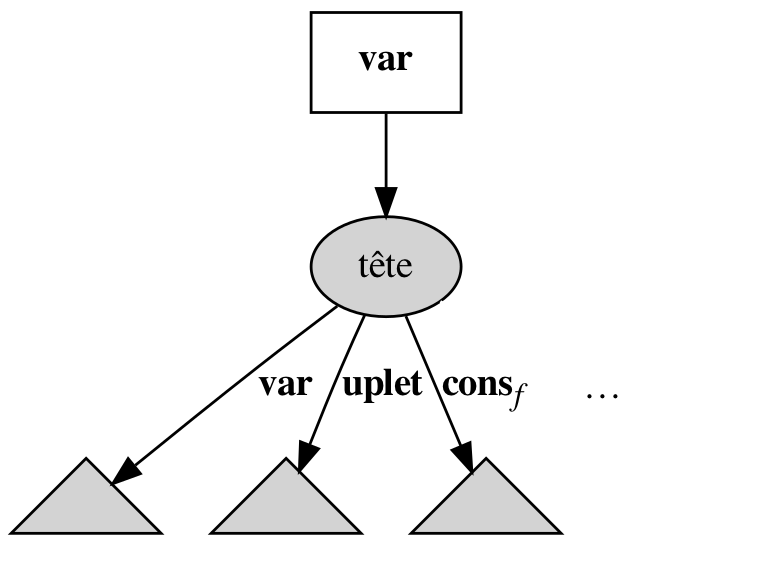
\includegraphics[scale=0.13]{graphs/crit1_1}
    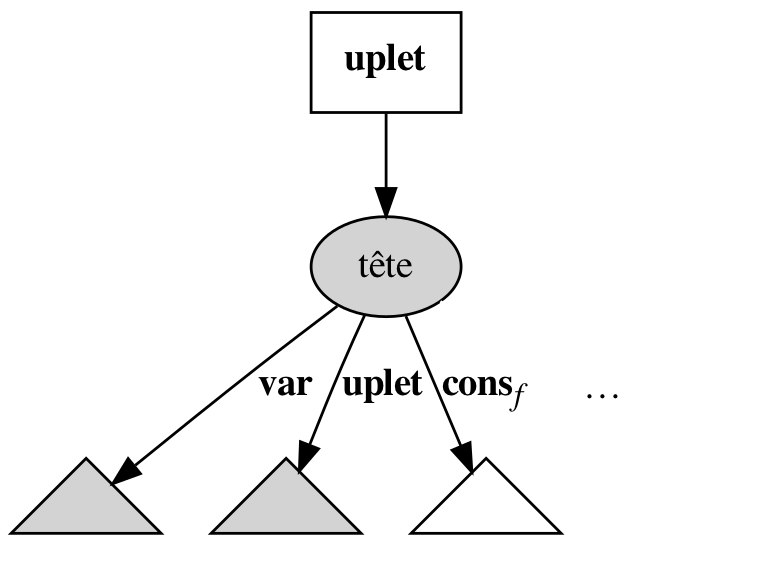
\includegraphics[scale=0.13]{graphs/crit1_2}
    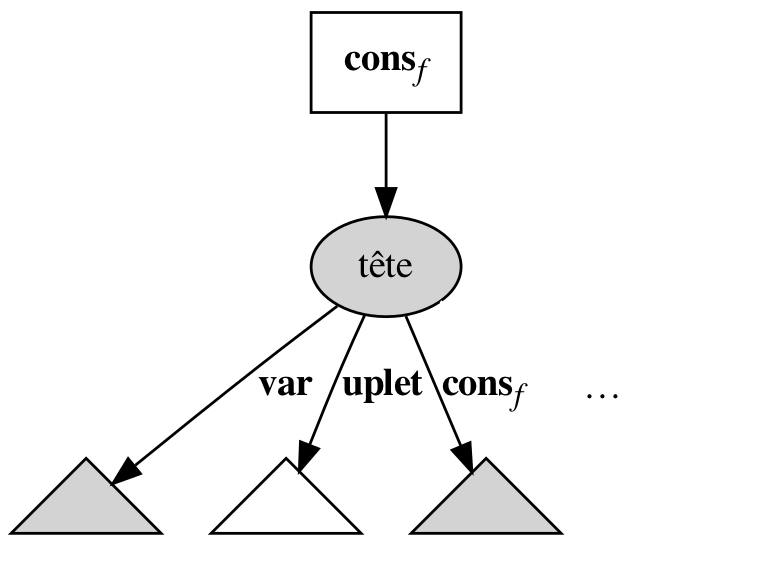
\includegraphics[scale=0.13]{graphs/crit1_3}
  \end{center}
  \caption{\label{fig_crit1}}
\end{figure}

\subsubsection{Apport}

Voyons ce qu'apporte ce premier critère en pratique. Nous avons collecté dans la table \ref{tab_apport1} les résultats de plusieurs requêtes. Les deuxième et troisième colonnes donnent le temps total d'unification sans et avec le critère ; il en est de même pour les quatrième et cinquième avec le nombre d'unifications. On peut obtenir ces données à l'aide des commandes (il n'y a pas besoin de répéter la première) :

\begin{verbatim}
$ ./dowsindex save --index index.db --features head
$ ./dowsindex stats --index index.db --features head --with-features <type>
\end{verbatim}

\begin{table}[h]
  \centering
  \begin{tabular}{|*{5}{c|}}
    \hline
      type &
      \multicolumn{2}{c|}{temps total ($s$)} &
      \multicolumn{2}{c|}{nb. d'unifications}
    \\
    \cline{2-5}
      &
      sans critère & avec critère &
      sans critère & avec critère
    \\
    \hline
      $int \rightarrow int \rightarrow int$ &
      0.63 & 0.08 (12.1\%) &
      31578 & 2714 (8.6\%)
    \\
      $int \rightarrow int \rightarrow int \rightarrow int$ &
      1.08 & 0.88 (81.4\%) &
      31578 & 2714 (8.6\%)
    \\
      $int \rightarrow (int \rightarrow int) \rightarrow list (\alpha)$ &
      1.09 & 0.29 (26.4\%) &
      31578 & 2945 (9.3\%)
    \\
      $int \rightarrow float \rightarrow bool \rightarrow \bold{unit}$ &
      0.31 & 0.17 (53.6\%) &
      31578 & 5745 (18.2\%)
    \\
      $\alpha \rightarrow int \rightarrow \bold{unit}$ &
      0.83 & 0.30 (36.4\%) &
      31578 & 5745 (18.2\%)
    \\
      $int \rightarrow int \rightarrow \alpha$ &
      5.77 & 5.43 (94.1\%) &
      31578 & 31578 (100\%)
    \\
    \hline
  \end{tabular}
  \caption{\label{tab_apport1}}
\end{table}

Premier constat : le critère se comporte comme prévu. Deux types distincts mais dont les têtes ont le même genre unifient autant de fois et la requête présentant une variable en tête ne profite pas du critère.

Deuxième constat : pour la plupart des requêtes, ce premier critère assez simple diminue considérablement le nombre d'unifications — entre 81.8\% et 91.4\% sont éliminées. Tant que la requête n'a pas de variable en tête, on peut tirer pleinement parti du fait que 95\% des types de l'environnement partagent cette caractéristique.

Le plus satisfaisant est de noter que le potentiel estimé à l'aide de la deuxième métrique se réalise par un critère intéressant. L'approche que nous avons adoptée en est corroborée.

%============================================================

\subsection{Deuxième critère}

\subsubsection{Présentation}

Le deuxième critère est plus sophistiqué que le premier. Observons plusieurs cas.

Plaçons-nous tout d'abord dans le cas où les deux types à unifier n'ont pas de variables à la base. Il vient aisément que, non seulement leurs têtes doivent avoir le même genre, mais on doit aussi trouver dans chaque queue les genres en quantités égales.

Plaçons-nous maintenant dans le cas où un seul des deux types possède cette caractéristique. Intuitivement, une variable de la base peut « absorber » des paramètres afin d'unifier — ce qui ne peut se produire dans un type en étant dépourvu. Ainsi, l'idée est que chaque genre non-variable représenté dans la queue d'un type quelconque doit nécessairement trouver son pareil au moins autant de fois dans la queue d'un type n'ayant pas cette capacité d'absorption.

Dans le dernier cas — le moins fréquent —, on ne peut rien affirmer.

Afin de formaliser la condition nécessaire résultante, on définit la notion de \emph{multiplicité}, qui compte le nombre de types d'un genre donné dans la queue d'un type :

\begin{definition}[multiplicité d'un genre dans un type normalisé]
  La multiplicité d'un genre $g$ dans un type normalisé $\nu$, notée $\mu_g (\nu)$, est définie par :
  \begin{align*}
      \mu_g (\nu^\# \rightarrow \nu) &=
      \mu_g' (\nu^\#)
    \\
      \mu_g (\nu) &=
      0
    \\
      \mu_g' (\mset{\nu_1, \dots, \nu_n}) &=
      \sum_{i=1}^n \mu_g'' (\nu_i)
    \\
      \mu_g'' (\nu) &=
      1 &&
      \text{si } [\nu] = g
    \\
      \mu_g'' (\nu) &=
      0 &&
      \text{sinon}
  \end{align*}
\end{definition}

Introduisons également les \emph{types normalisés simples}. Il s'agit des types ne possédant pas de variables à la base. Nous avons vu que neuf dixièmes des types de l'environnement sont simples. A cela s'ajoute le fait que le motif du matching est toujours simple.

\begin{definition}[type normalisé simple]
  Le prédicat sur les types normalisés « est simple », noté $\bold{simple}$, est défini par :
  \begin{mathpar}
    \inferrule*
      {[\nu] \notin \{ \bold{var}, \bold{fleche} \}}
      {\nu\ \bold{simple}}
    \and
    \inferrule*
      {\forall i \in \interval 1 n,\ [\nu_i] \neq \bold{var} \\ [\nu] \neq \bold{var}}
      {\mset{\nu_1, \dots, \nu_n} \rightarrow \nu\ \bold{simple}}
  \end{mathpar}
\end{definition}

Bien qu'intéressante dans le cadre des démonstrations, cette définition n'est pas adaptée à l'implémentation. Pour décider si un type est simple, on utilisera la métrique $\mu^3$ :

\begin{lemme}
  Un type normalisé est simple \ssi sa mesure au sens de $\mu^3$ est nulle.
\end{lemme}

\begin{preuve}
  Les deux sens se démontrent sans difficulté.
\end{preuve}

Ces définitions étant posées, nous sommes en mesure d'exprimer la seconde condition nécessaire :

\begin{theoreme} \label{thm_cond2}
  Si deux types normalisés bien formés $\nu_1$ et $\nu_2$ sont unifiables et $\nu_1$ simple, la multiplicité de tout genre différent de $\bold{var}$ dans $\nu_1$ est supérieure ou égale à celle dans $\nu_2$.
\end{theoreme}

\begin{preuve}
	Voir annexe.
\end{preuve}

\begin{exemple}
  Par contraposée, les types suivants ne sont pas unifiables :
  \begin{itemize}
    \item $\mset{int, int} \rightarrow int$ et $\mset{int} \rightarrow float$ ;
    \item $\mset{int} \rightarrow int$ et $\mset{int, int, \alpha} \rightarrow \alpha$ ;
    \item $\mset{int, \mset{} \rightarrow \mset{}} \rightarrow \mset{}$ et $\mset{int, \mset{int} \rightarrow float, int} \rightarrow \alpha$.
  \end{itemize}
\end{exemple}

\subsubsection{Implémentation}

Quant à l'implémentation, on peut d'abord exprimer le critère résultant pour chaque genre adéquat. De même que précédemment, on le représente visuellement par des arbres de décision en figure \ref{fig_crit2}.

\begin{definition}[$\mathrm{crit}^2_g$]
  Soit un genre de types normalisés $g$ différent de $\bold{var}$ et $\bold{uplet}$. \\
  On note $\mathrm{crit}^2_g$ le critère $(\mathrm{encode}^2_g, \mathrm{compat}^2_g)$ sur $\mathscr{D}^2_{g} = \mathbb{B} \times \mathbb{N}$, où $\mathrm{encode}^2_g$ et $\mathrm{compat}^2_g$ sont définies par :
  \begin{align*}
      \mathrm{encode}^2_g (\nu) &=
      (\mathrm{vars\mathhyphen base} (\nu), \mu_g (\nu))
    \\
      \mathrm{vars\mathhyphen base} (\nu) &=
      \bold{F} &&
      \text{si } \mu^3 (\nu) = 0
    \\
      \mathrm{vars\mathhyphen base} (\nu) &=
      \bold{V} &&
      \text{sinon}
  \end{align*}
  \begin{align*}
      \mathrm{compat}^2_g ((\bold{V}, \mu_1), (\bold{V}, \mu_2)) &=
      \bold{V}
    \\
      \mathrm{compat}^2_g ((\bold{V}, \mu_1), (\bold{F}, \mu_2)) &=
      \bold{V} &&
      \text{si } \mu_1 \leqslant \mu_2
    \\
      \mathrm{compat}^2_g ((\bold{V}, \mu_1), (\bold{F}, \mu_2)) &=
      \bold{F} &&
      \text{sinon}
    \\
      \mathrm{compat}^2_g ((\bold{F}, \mu_1), (\bold{V}, \mu_2)) &=
      \bold{V} &&
      \text{si } \mu_2 \leqslant \mu_1
    \\
      \mathrm{compat}^2_g ((\bold{F}, \mu_1), (\bold{V}, \mu_2)) &=
      \bold{F} &&
      \text{sinon}
  \end{align*}
\end{definition}

\begin{figure}[h]
  \begin{center}
    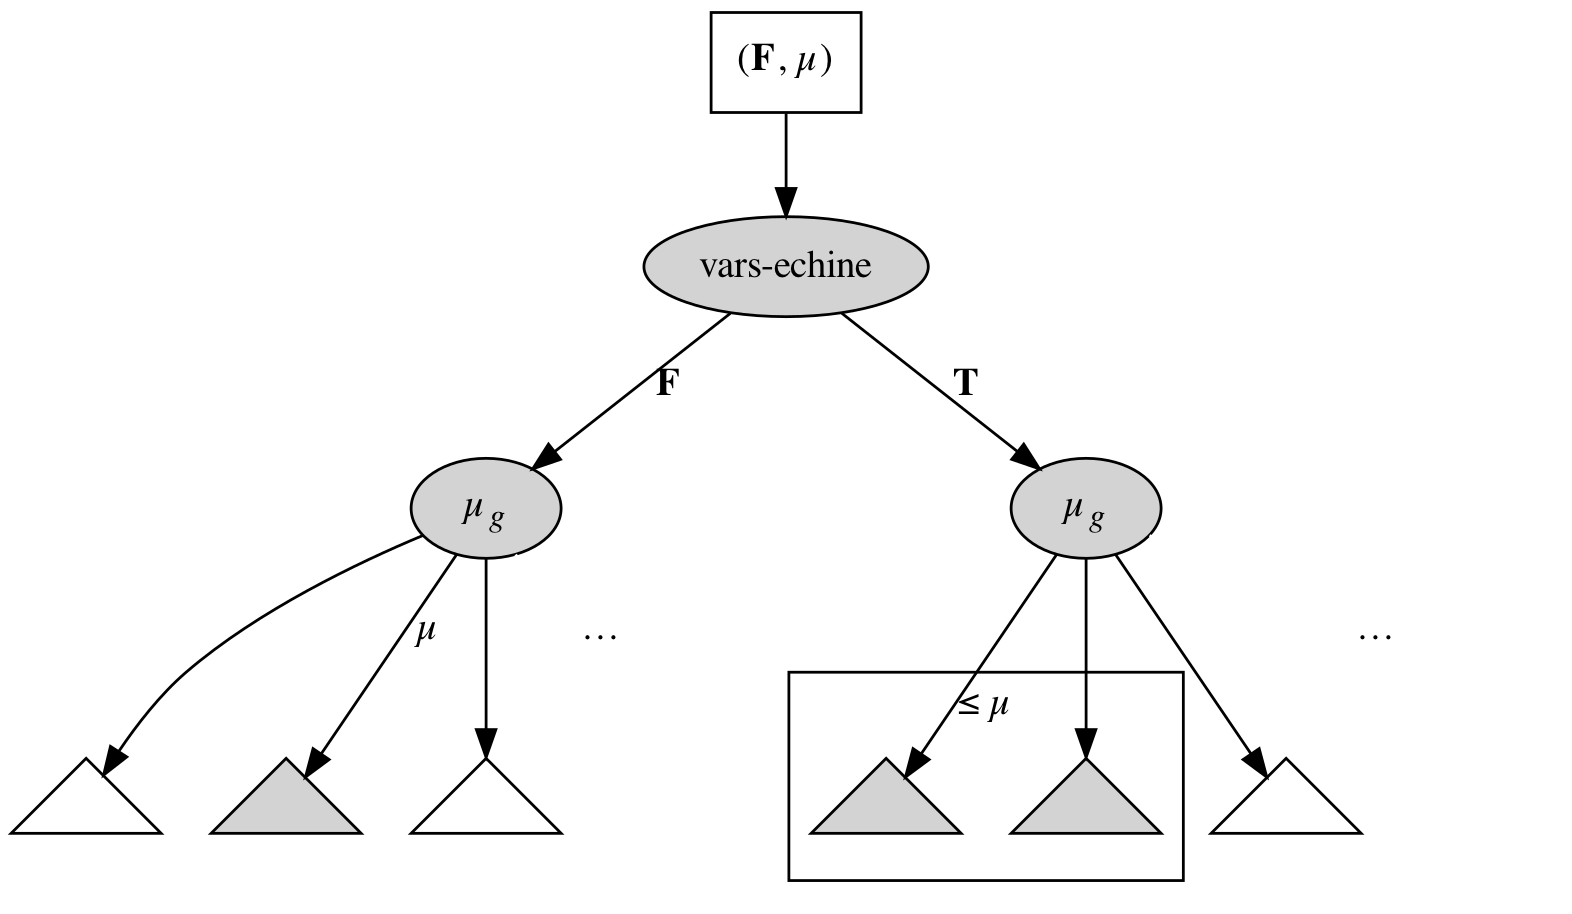
\includegraphics[scale=0.13]{graphs/crit2_1}
    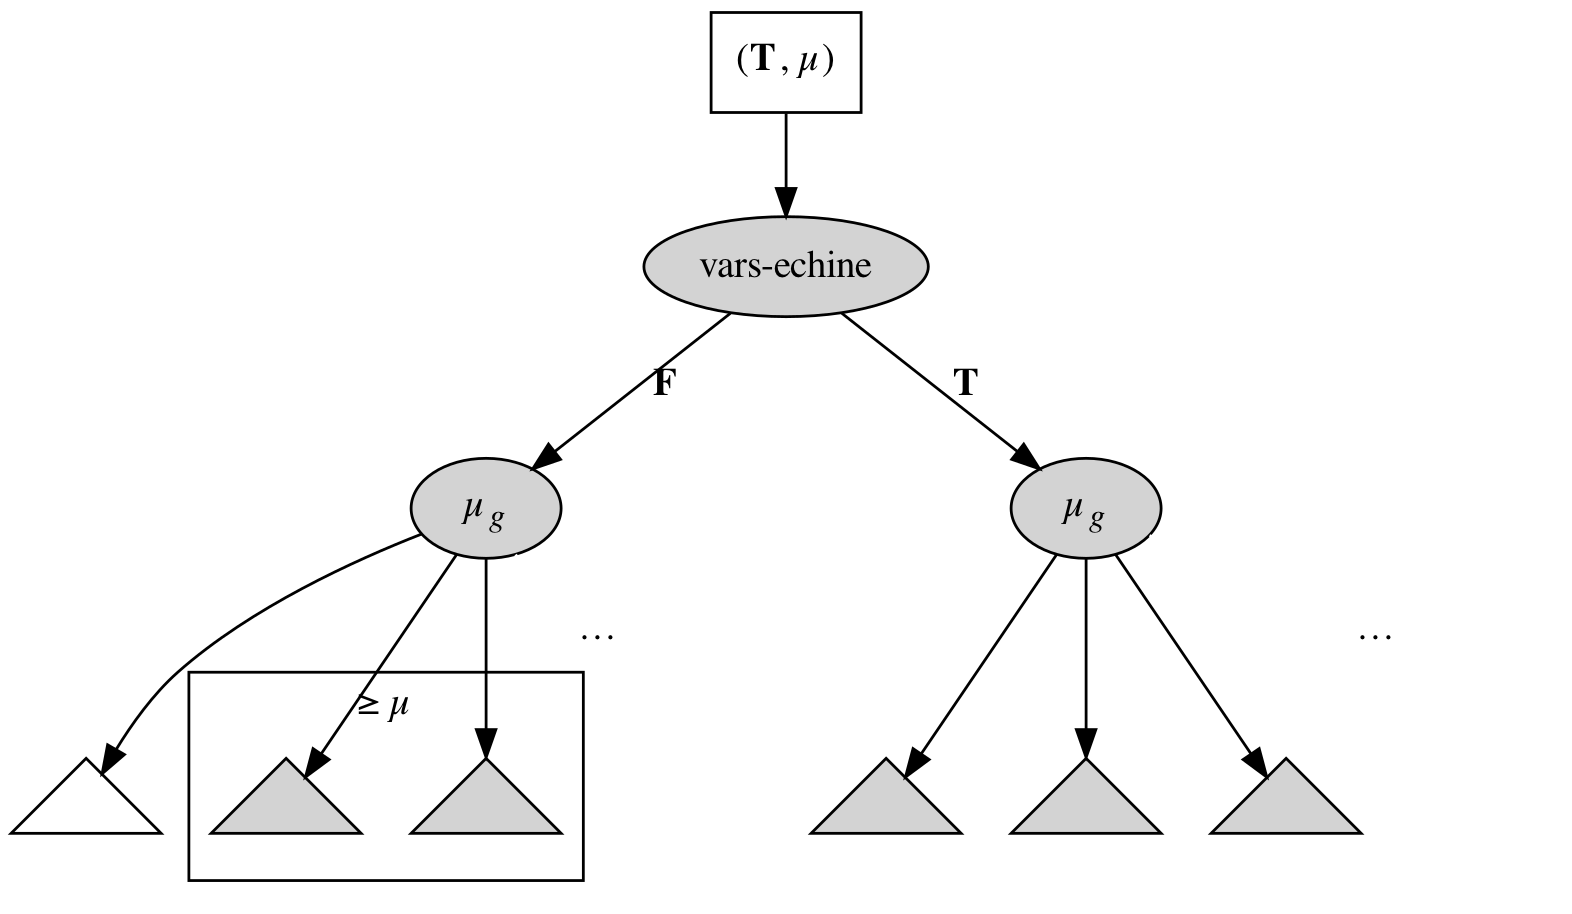
\includegraphics[scale=0.13]{graphs/crit2_2}
  \end{center}
  \caption{\label{fig_crit2}}
\end{figure}

\begin{theoreme} \label{thm_crit2g}
  Pour tout genre $g$ différent de $\bold{var}$ et $\bold{uplet}$, le critère d'unifiabilité $\mathrm{crit}^1_g$ est correct.
\end{theoreme}

\begin{preuve}
  Par le théorème \ref{thm_cond2}.
\end{preuve}

Cependant, introduire autant de critères qu'il y a de constructeurs de types n'est pas une bonne idée. En fait, on peut « paralléliser » tous ces critères en travaillant sur des multi-ensembles de genres. Les inégalités ci-dessus laissent place à des inclusions entre multi-ensembles.

\begin{definition}[$\mathrm{crit}^2$]
  On note $\mathrm{crit}^2$ le critère $(\mathrm{encode}^2, \mathrm{compat}^2)$ sur $\mathscr{D}^2 = \mathbb{B} \times \G^\#$, où $\mathrm{encode}^2$ et $\mathrm{compat}^2$ sont définies par :
  \[ \mathrm{encode}^2 (\nu) = \left( \mathrm{vars\mathhyphen base} (\nu), \msetG_bigplus_{g \notin \{ \bold{var}, \bold{uplet} \}} \msetG_bigplus_{\interval 1 {\mu_g (\nu)}} \mset{g} \right) \]
  \begin{align*}
      \mathrm{compat}^2 ((\bold{V}, {g}^\#_1), (\bold{V}, {g}^\#_2)) &=
      \bold{V}
    \\
      \mathrm{compat}^2 ((\bold{V}, {g}^\#_1), (\bold{F}, {g}^\#_2)) &=
      \bold{V} &&
      \text{si } {g}^\#_1 \subseteq^\#_\G {g}^\#_2
    \\
      \mathrm{compat}^2 ((\bold{V}, {g}^\#_1), (\bold{F}, {g}^\#_2)) &=
      \bold{F} &&
      \text{sinon}
    \\
      \mathrm{compat}^2 ((\bold{F}, {g}^\#_1), (\bold{V}, {g}^\#_2)) &=
      \bold{V} &&
      \text{si } {g}^\#_2 \subseteq^\#_\G {g}^\#_1
    \\
      \mathrm{compat}^2 ((\bold{F}, {g}^\#_1), (\bold{V}, {g}^\#_2)) &=
      \bold{F} &&
      \text{sinon}
  \end{align*}
\end{definition}

\begin{theoreme} \label{thm_crit2}
  Le critère d'unifiabilité $\mathrm{crit}^2$ est correct.
\end{theoreme}

\begin{preuve}
  On interprète l'inclusion sur les multi-ensembles en termes de multiplicités. Le résultat se déduit du théorème \ref{thm_crit2g}.
\end{preuve}

\subsubsection{Apport}

Allions les deux critères. Les résultats sont présentés en table \ref{tab_apport2}. Ils ont été obtenus grâce à la commande suivante :

\begin{verbatim}
$ ./dowsindex stats --with-features <type>
\end{verbatim}

\begin{table}[h]
  \centering
  \begin{tabular}{|*{5}{c|}}
    \hline
      type &
      \multicolumn{2}{c|}{temps total ($s$)} &
      \multicolumn{2}{c|}{nb. d'unifications}
    \\
    \cline{2-5}
      &
      sans critères & avec critères &
      sans critères & avec critères
    \\
    \hline
      $int \rightarrow int \rightarrow int$ &
      0.638 & 0.001 (0.23\%) &
      31578 & 121 (0.38\%)
    \\
      $int \rightarrow int \rightarrow int \rightarrow int$ &
      1.622 & 0.001 (0.08\%) &
      31578 & 107 (0.34\%)
    \\
      $int \rightarrow (int \rightarrow int) \rightarrow list (\alpha)$ &
      11.193 & 0.011 (0.93\%) &
      31578 & 141 (0.45\%)
    \\
      $int \rightarrow float \rightarrow bool \rightarrow \bold{unit}$ &
      0.636 & 0.004 (0.60\%) &
      31578 & 126 (0.40\%)
    \\
      $\alpha \rightarrow int \rightarrow \bold{unit}$ &
      1.180 & 0.225 (19.06\%) &
      31578 & 2443 (7.74\%)
    \\
      $int \rightarrow int \rightarrow \alpha$ &
      5.097 & 1.566 (30.71\%) &
      31578 & 3677 (11.64\%)
    \\
    \hline
  \end{tabular}
  \caption{\label{tab_apport2}}
\end{table}

Force est de constater que les critères fonctionnent très bien sur ces requêtes. Les plus simples sont traitées de façon instantanée. Il est satisfaisant de constater que l'unification sur un environnement de dizaines de millers de types se réduit dans ces cas à quelques centaines seulement.

Au vu de ces faibles résidus, on peut raisonnablement affirmer avoir épuisé les cas simples. Un troisième critère devrait se confronter à des types plus retors.

%============================================================
%============================================================

\section{Utilisation d'un trie}

Nous avons à présent tous les éléments pour construire un \emph{index}. On est naturellement confronté au choix de la structure de données à employer. L'idée de Gabriel Radanne, inspirée par \cite{Schulz}, est d'adapter la structure de \emph{trie} aux critères.

Les tries servent à stocker efficacement une table associative où les clefs sont des mots sur un alphabet donné. Ce n'est pas le cas ici. Nous travaillons plutôt sur la concaténation des codes des deux critères, dans laquelle est contenue toute l'information nécessaire aux tests de compatibilité. Ces derniers compliquent d'ailleurs la chose : plusieurs branches peuvent être compatibles avec la requête (voir les figures \ref{fig_crit1} et \ref{fig_crit2}). En somme, il faut revoir la structure.

En première approximation, notre structure consiste en un arbre dont les nœuds internes sont étiquetés par des critères et les feuilles par des ensembles de types. On la définit ainsi :

\begin{definition}[tries de types normalisés]
  L'ensemble des tries de types normalisés, noté $\mathscr{T}$, est défini inductivement par :
  \begin{mathpar}
    \inferrule*
      {N \subseteq \N}
      {\bold{feuille} (N) \in \mathscr{T}}
    \and
    \inferrule*
      {crit \in \mathscr{C}_\mathscr{D} \\ fils \in \mathscr{F} (\mathscr{D}, \mathscr{T})}
      {\bold{noeud}_\mathscr{D} (crit, fils) \in \mathscr{T}}
  \end{mathpar}
\end{definition}

\begin{exemple}
  Avec nos deux critères, le trie vide s'écrit : \\
  \[ \bold{noeud}_{\mathscr{D}^1} (\mathrm{crit}^1, g \mapsto \bold{noeud}_{\mathscr{D}^2} (\mathrm{crit}^2, (b, g^\#) \mapsto \bold{feuille} (\{ \}))) \]
\end{exemple}

On les manipule à l'aide de deux fonctions. La première ajoute un type à un trie par un appel récursif sur le sous-arbre associé au code du type ajouté.

\begin{definition}[$\mathrm{trie\mathhyphen ajoute}$]
  La fonction $\mathrm{trie\mathhyphen ajoute}$ est définie récursivement par :
  \begin{align*}
      \mathrm{trie\mathhyphen ajoute} (\bold{feuille} (N), \nu) &=
      \bold{feuille} (N \cup \{ \nu \})
    \\
      \mathrm{trie\mathhyphen ajoute} (\bold{noeud}_\mathscr{D} (crit, fils), \nu) &=
      \bold{noeud}_\mathscr{D} (crit, d \mapsto \mathrm{trie\mathhyphen ajoute}_\mathscr{D}' (crit, fils, \nu, d))
  \end{align*}
  \begin{align*}
      \mathrm{trie\mathhyphen ajoute}_\mathscr{D}' ((encode, \_), fils, \nu, d) &=
      \mathrm{trie\mathhyphen ajoute} (fils (d), \nu) &&
      \text{si } d = encode (\nu)
    \\
      \mathrm{trie\mathhyphen ajoute}_\mathscr{D}' ((encode, \_), fils, \nu, d) &=
      fils (d) &&
      \text{sinon}
  \end{align*}
\end{definition}

La seconde calcule l'ensemble des types d'un trie compatibles pour tous les critères avec une requête donnée. Elle consiste en un appel récursif sur les sous-arbres compatibles avec la requête.

\begin{definition}[$\mathrm{trie\mathhyphen cherche}$]
  La fonction $\mathrm{trie\mathhyphen cherche}$ est définie récursivement par :
  \begin{align*}
      \mathrm{trie\mathhyphen cherche} (\bold{feuille} (N), \nu) &=
      N
    \\
      \mathrm{trie\mathhyphen cherche} (\bold{noeud}_\mathscr{D} ((encode, compat), fils), \nu) &=
      \bigcup_{\mathclap{{d \in \mathscr{D} \mid compat (d, encode (\nu)) = \bold{T}}}} \mathrm{trie\mathhyphen cherche} (fils (d), \nu)
  \end{align*}
\end{definition}

L'interface de implémentation OCaml correspondante est présentée ci-dessous. On y retrouve les fonctions d'encodage et de test de compatibilité des critères — \mintinline{ocaml}{compute} et \mintinline{ocaml}{compatible} — la structure arborescente avec feuilles et nœuds — \mintinline{ocaml}{Leaf} et \mintinline{ocaml}{Node} — ainsi que les fonctions d'ajout et de recherche — \mintinline{ocaml}{add} et \mintinline{ocaml}{iter_with}. La fonction \mintinline{ocaml}{compare} définit un ordre total sur les critères dont \mintinline{ocaml}{Node} a besoin pour ses structures de données. \mintinline{ocaml}{empty} est le trie vide.

Sa simplicité est particulièrement appréciable. Il est aisé d'ajouter et expérimenter de nouveaux critères.

\begin{minted}{ocaml}
module type FEATURE = sig
  type t
  val compute : Type.t -> t
  val compare : t -> t -> Int.t
  val compatible : query:t -> data:t -> Bool.t
end

module type NODE = sig
  type t
  val empty : t
  val add : Type.t -> t -> t
  val iter_with : Type.t -> t -> Type.t Iter.t
end

module Leaf : NODE
module Node (Feat : FEATURE) (Sub : NODE) : NODE
\end{minted}

%============================================================
%============================================================
%============================================================

\chapter{\dowsindex}

Dans ce dernier chapitre, nous visitons les fonctionnalités du programme \dowsindex. On pourra en trouver le code source sur le dépôt \textit{github} \href{https://github.com/Drup/dowsing}{\texttt{Drup/dowsing}}. La version actuelle est compatible avec les systèmes d'exploitation Linux et macOS.

\dowsindex met en application les techniques présentées dans le chapitre précédent. Avant toute chose, il faut donc créer un \emph{index} auquel \dowsindex se référera au moment de la recherche. La commande suivante fait l'affaire :

\begin{verbatim}
$ dowsindex save
\end{verbatim}

L'index est entreposé dans un répertoire standard destiné aux données d'applications. On peut aussi indiquer explicitement où le sauvegarder :

\begin{verbatim}
$ dowsindex save --index <fichier>
\end{verbatim}

On peut également préciser quels paquets OPAM inclure dans l'index — notamment afin de réduire le temps de construction. La command suivante a cet effet, mais aussi — si l'index existe déjà — celui de charger ou recharger les paquets désignés :

\begin{verbatim}
$ dowsindex save [--index <fichier>] <paquet>...
\end{verbatim}

Ceci étant fait — et une bonne fois pour toutes —, on peut maintenant utiliser \dowsindex pour sa fin première : recherche une fonction par son type. Si l'index a été créé dans le répertoire standard, il suffit de demander :

\begin{verbatim}
$ dowsindex search <type>
\end{verbatim}

Sinon, il faut préciser le chemin de l'index :

\begin{verbatim}
$ dowsindex search --index <fichier> <type>
\end{verbatim}

Si tout se passe bien, le programme affiche la liste des fonctions retenues avec leurs types. Pour ne garder que les $n$ premières réponses, on peut employer l'option \texttt{-n} :

\begin{verbatim}
$ dowsindex search [--index <fichiers>] -n <n> <type>
\end{verbatim}

L'espace de recherche peut être limité à certains paquets — c'est d'ailleurs le scénario le plus courant — :

\begin{verbatim}
$ dowsindex search [--index <fichiers>] [-n <n>] <paquet>... <type>
\end{verbatim}

On peut par exemple rechercher une fonction de la bibliothèque standard testant l'appartenance à une liste :

\begin{verbatim}
$ ./dowsindex search stdlib "'a list * 'a -> bool"
Parsing.is_current_lookahead : 'a -> bool
Obj.magic : 'a -> 'b
List.mem : 'a -> 'a list -> bool
List.memq : 'a -> 'a list -> bool
ListLabels.mem : 'a -> set:'a list -> bool
ListLabels.memq : 'a -> set:'a list -> bool
Compenv.print_version_string : unit -> 'a
Compenv.print_standard_library : unit -> 'a
\end{verbatim}

Mentionnons une dernière fonctionnalité. Par défaut, \dowsindex fait du \emph{matching} (voir chapitre 2). Pour les requêtes non polymorphes, cela revient à unifier. Pour les requêtes polymorphes, cela signifie que les variables sont chacune remplacées avant unification par une constante fraîche — n'apparaissant pas dans l'environnement — qui leur est propre. Sous cette nouvelle apparence, elles ne sont unifiables qu'avec des variables ; autrement dit, cela force le polymorphisme. C'est généralement le comportement souhaité. Néanmoins, l'utilisateur peut formuler sa requête sous la forme plus générale d'un \emph{schéma de types}. Les variables polymorphes non instanciables y sont spécifiées avant le type, les deux étant séparés d'un point ; les autres variables libres du type seront alors instanciables. En résumé, \dowsindex accepte la syntaxe suivante :

\[ \T \mid \V \dots \V \texttt{.} \T \]

On peut par exemple demander :

\begin{verbatim}
$ dowsindex search "a b. ('a -> 'b -> 'a) -> 'a -> 'b list -> 'a"
\end{verbatim}

Les deux variables étant explicitement liées, cela revient à :

\begin{verbatim}
$ dowsindex search "('a -> 'b -> 'a) -> 'a -> 'b list -> 'a"
\end{verbatim}

En revanche, les variables de cette requête sont instanciables car non liées :

\begin{verbatim}
$ dowsindex search ". ('a -> 'b -> 'a) -> 'a -> 'b list -> 'a"
\end{verbatim}

%============================================================
%============================================================
%============================================================

\chapter{Conclusion}

Nous arrivons au terme de ce rapport. Retraçons ses grandes lignes. A partir d'une implémentation de l'\emph{unification modulo isomorphismes de types}, nous avons amené, défini et démontré deux \emph{critères d'unifiabilité}. Ces critères sont utilisés par \dowsindex dans la construction d'un \emph{index}. Ce travail permet de réduire significativement le nombre d'appels à l'unification. Les requêtes les plus simples sont traitées de façon instantanée.

Il y a encore à faire : terminer les preuves, définir d'autres critères visant les cas plus difficiles, prendre en compte des types OCaml plus sophistiqués\dots Plusieurs aspects de l'indexation mériteraient qu'on s'y arrête : récupération des fonctions de l'environnement OPAM, sauvegarde et chargement de l'index (pour le moment réalisés avec le module \mintinline{ocaml}{Marshall}). \dowsindex souffre particulièrement du fait que la qualification des types par rapport au module englobant est mal assurée ; par exemple, la fonction \mintinline{ocaml}{Format.pp_print_int} est connue sous le type \mintinline{ocaml}{formatter -> int -> unit}, et non pas \mintinline{ocaml}{Format.formatter -> int -> unit}.

Quoi qu'il en soit, nous espérons avoir posé de solides bases au système \dowsindex. Je remercie Gabriel Radanne et Laure Gonnord pour leur encadrement tout au long du stage. Je ne remercie pas le SARS-CoV-2 pour les conditions particulières dans lesquelles il s'est déroulé.

%============================================================
%============================================================
%============================================================

\chapter*{Annexe}
\addcontentsline{toc}{chapter}{Annexe}

Cette annexe est dévolue aux démonstrations des deux conditions nécessaires d'unifiabilité.

%============================================================
%============================================================

\section{Première condition nécessaire}

\begin{theoreme} \label{thm_cond1}
  Si deux types normalisés bien formés sont unifiables et que leurs têtes ne sont pas des variables, elles ont le même genre.
\end{theoreme}

\begin{preuve}
  Par hypothèse, il existe $\theta$ dans $\Theta$ telle que :
  \[ \hat\theta (\nu_1) = \hat\theta (\nu_2) \]
  On passe à la tête dans cette égalité :
  \[ \uparrow \hat\theta (\nu_1) =\ \uparrow \hat\theta (\nu_2) \]
  Le lemme \ref{tete_subst_eq_tete_subst_tete} donne :
  \[ \uparrow \hat\theta (\uparrow \nu_1) =\ \uparrow \hat\theta (\uparrow \nu_2) \]
  Soit $i$ dans $\{ 1, 2 \}$. \\
  Par hypothèse, la tête de $\nu_i$ n'est pas une variable. Le lemme \ref{non_var_implique_subst_preserve_genre} nous assure donc que :
  \[ [ \hat\theta (\uparrow \nu_i) ] = [ \uparrow \nu_1 ] \]
  Par hypothèse, $\nu_i$ est bien formé. Par le lemme \ref{bf_implique_tete_bf_et_non_fleche}, sa tête n'est pas une flèche et donc, d'après la remarque précédente, $\hat\theta (\uparrow \nu_i)$ non plus. Par le lemme \ref{non_fleche_implique_tete_preserve_genre}, on a ainsi :
  \[ [ \uparrow \hat\theta (\uparrow \nu_i) ] = [ \hat\theta (\uparrow \nu_i) ] = [ \uparrow \nu_i ] \]
  On en déduit le résultat attendu.
\end{preuve}

\begin{lemme} \label{tete_subst_eq_tete_subst_tete}
  Pour tout $\nu$ dans $\N$ et $\theta$ dans $\Theta$, on a :
  \[ \uparrow \hat\theta (\nu) =\ \uparrow \hat\theta (\uparrow \nu) \]
\end{lemme}

\begin{preuve}
  Par cas sur le type. \\
  Seul le cas flèche est non trivial : $\nu^\# \rightarrow \nu$. \\
  Par définition de $\uparrow \cdot$, on a d'abord :
  \[ \uparrow \hat\theta (\uparrow (\nu^\# \rightarrow \nu)) =\ \uparrow \hat\theta (\nu) \]
  \begin{itemize}[label={\textbf{Si}}]
    \item 
      $\hat\theta (\nu) = {\nu^\#}' \rightarrow \nu'$ : \\
      Par définition de $\hat\theta$ et $\uparrow \cdot$, on a d'une part :
      \[ \uparrow \hat\theta (\nu^\# \rightarrow \nu) = \nu' \]
      Par définition de $\uparrow \cdot$, on a d'autre part :
      \[ \uparrow \hat\theta (\nu) = \nu' \]
      On en déduit le résultat.
    \item 
      non : \\
      Par définition de $\hat\theta$ et $\uparrow \cdot$, on a :
      \[ \uparrow \hat\theta (\nu^\# \rightarrow \nu) = \hat\theta (\nu) \]
      Le résultat se déduit du fait que $\hat\theta (\nu)$ n'est pas une flèche.
  \end{itemize}
\end{preuve}

\begin{lemme} \label{non_var_implique_subst_preserve_genre}
  L'application d'une substitution étendue à un type normalisé qui n'est pas une variable préserve son genre.
\end{lemme}

\begin{preuve}
  Trivial avec la définition de l'extension d'une substitution.
\end{preuve}

\begin{lemme} \label{non_fleche_implique_tete_preserve_genre}
  La tête d'un type normalisé qui n'est pas une flèche préserve son genre.
\end{lemme}

\begin{preuve}
  Trivial avec la définition de la tête.
\end{preuve}

%============================================================
%============================================================

\section{Deuxième condition nécessaire}

\begin{theoreme} \label{thm_cond2}
  Si deux types normalisés bien formés $\nu_1$ et $\nu_2$ sont unifiables et $\nu_1$ simple, la multiplicité de tout genre différent de $\bold{var}$ dans $\nu_1$ est supérieure ou égale à celle dans $\nu_2$.
\end{theoreme}

\begin{preuve}
  Soit $g$ dans $\G$ différent de $\bold{var}$. \\
  Par hypothèse, il existe $\theta$ dans $\Theta$ telle que :
  \[ \hat\theta (\nu_1) = \hat\theta (\nu_2) \]
  On passe aux multiplicités dans cette égalité :
  \[ \mu_g (\hat\theta (\nu_1)) = \mu_g (\hat\theta (\nu_2)) \]
  Par le lemme \ref{bf_simple_implique_mu_eq_mu_subst}, on a d'une part :
  \[ \mu_g (\hat\theta (\nu_1)) = \mu_g (\nu_1) \]
  Par le lemme \ref{bf_implique_mug_subst_geq_mug}, on a d'autre part :
  \[ \mu_g (\hat\theta (\nu_2)) \geqslant \mu_g (\nu_2) \]
  On en déduit le résultat attendu.
\end{preuve}

\begin{lemme} \label{genre_eq_implique_mug''_eq}
  Soient $\nu_1$ et $\nu_2$ dans $\N$ de même genre. Pour tout genre $g$, on a :
  \[ \mu_g'' (\nu_1) = \mu_g'' (\nu_2) \]
\end{lemme}

\begin{preuve}
  Trivial avec la définition de $\mu_g''$.
\end{preuve}

\begin{lemme} \label{bf_simple_implique_mu_eq_mu_subst}
  Soient $\nu$ dans $\N^{\bold{bf}}$ simple, $g$ dans $\G$ différent de $\bold{var}$ et $\theta$ dans $\Theta$. La multiplicité de $g$ dans $\nu$ est la même que dans $\hat\theta (\nu)$.
\end{lemme}

\begin{preuve}
  Par cas sur le type. \\
  Seul le cas flèche est non trivial : $\nu^\# \rightarrow \nu$, avec $\nu^\# = \mset{\nu_1, \dots, \nu_n}$. \\
  Par hypothèse de simplicité et bonne formation, le genre de $\nu$ est différent de $\bold{var}$ et $\bold{fleche}$. \\
  Par le lemme \ref{non_var_implique_subst_preserve_genre}, le genre de $\hat\theta (\nu)$ est donc différent de $\bold{fleche}$. \\
  Il vient alors par définition de $\hat\theta$ :
  \[ \hat\theta (\nu^\# \rightarrow \nu) = \tilde\theta (\nu^\#) \rightarrow \hat\theta (\nu) \]
  Par définition de $\mu_g$ et $\tilde\theta$, on a :
  \[ \mu_g (\hat\theta (\nu^\# \rightarrow \nu)) = \mu_g' \left( \msetN_bigplus_{i \in \interval 1 n} \norm' (\hat\theta (\nu_i)) \right) \]
  Par simplicité et bonne formation, tous les $\nu_i$ sont de genre différent de $\bold{var}$ et $\bold{uplet}$. \\
  Par le lemme \ref{non_var_implique_subst_preserve_genre}, on a donc :
  \[ \forall i \in \interval 1 n,\ [ \hat\theta (\nu_i) ] = [ \nu_i ] \neq \bold{uplet} \]
  Par définition de $\norm'$, cela implique :
  \[ \forall i \in \interval 1 n,\ \norm' (\hat\theta (\nu_i)) = \mset{\hat\theta (\nu_i)} \]
  On peut donc écrire :
  \[ \mu_g (\hat\theta (\nu^\# \rightarrow \nu)) = \mu_g' (\mset{\hat\theta (\nu_1), \dots, \hat\theta (\nu_n)}) = \sum_{i=1}^n \mu_g'' (\hat\theta (\nu_i)) \]
  Par le lemme \ref{genre_eq_implique_mug''_eq}, on a en outre :
  \[ \forall i \in \interval 1 n,\ \mu_g'' (\hat\theta (\nu_i)) = \mu_g'' (\nu_i) \]
  Ce qui nous donne :
  \[ \mu_g (\hat\theta (\nu^\# \rightarrow \nu)) = \sum_{i=1}^n \mu_g'' (\nu_i) = \mu_g' (\nu^\#) = \mu_g (\nu^\# \rightarrow \nu) \]
  C'est bien le résultat attendu.
\end{preuve}

\begin{lemme} \label{mug'_somme_eq_somme_mug'}
  Pour tous $\nu^\#_1$ et $\nu^\#_2$ dans $\N^\#$ et $g$ dans $\G$, on a :
  \[ \mu_g' (\nu^\#_1 +^\#_\N \nu^\#_2) = \mu_g' (\nu^\#_1) +^\#_\N \mu_g' (\nu^\#_2) \]
\end{lemme}

\begin{preuve}
  Trivial par définition de $\mu_g'$.
\end{preuve}

\begin{lemme} \label{non_uplet_implique_mug'_norm'_subst_geq_mug''}
  Pour tout $\nu$ dans $\N$ de genre différent de $\bold{uplet}$ et $g$ dans $\G$ différent de $\bold{var}$, on a :
  \[ \mu_g' (\norm' (\hat\theta (\nu))) \geqslant \mu_g'' (\nu) \]
\end{lemme}

\begin{preuve}
  Par hypothèse, $\nu$ n'est pas un uplet. Reste trois cas.
  \begin{itemize}[label={\textbf{Si}}]
    \item
      $\nu$ est une variable : trivial.
    \item
      non : \\
      Par le lemme \ref{non_var_implique_subst_preserve_genre}, $\hat\theta (\nu)$ est du même genre que $\nu$, différent de $\bold{uplet}$ par hypothèse. \\
      Par définition de $\norm'$ et $\mu_g'$, on a donc :
      \[ \mu_g' (\norm' (\hat\theta (\nu))) = \mu_g'' (\hat\theta (\nu)) \]
      Le lemme \ref{genre_eq_implique_mug''_eq} nous donne le résultat attendu :
      \[ \mu_g' (\norm' (\hat\theta (\nu))) = \mu_g'' (\nu) \]
  \end{itemize}
\end{preuve}

\begin{lemme} \label{pbf_implique_mug'_subst_geq_mug'}
  Pour tout $\nu^\#$ dans $\N^\#$ presque bien formé et $g$ dans $\G$ différent de $\bold{var}$, on a :
  \[ \mu_g' (\tilde\theta (\nu^\#)) \geqslant \mu_g' (\nu^\#) \]
\end{lemme}

\begin{preuve}
  Par définition de $\hat\theta$ et par le lemme \ref{mug'_somme_eq_somme_mug'}, il vient :
  \[ \mu_g' (\tilde\theta (\nu^\#)) = \sum_{i=1}^n \mu_g' (\norm' (\hat\theta (\nu_i))) \]
  $\nu^\#$ étant presque bien formé par hypothèse, tous les $\nu_i$ sont de genre différent de $\bold{uplet}$. \\
  Par le lemme \ref{non_uplet_implique_mug'_norm'_subst_geq_mug''}, on a donc :
  \[ \forall i \in \interval 1 n,\ \mu_g' (\norm' (\hat\theta (\nu_i))) \geqslant \mu_g'' (\nu_i) \]
  D'où le résultat attendu :
  \[ \mu_g' (\tilde\theta (\nu^\#)) \geqslant \sum_{i=1}^n \mu_g'' (\nu_i) = \mu_g' (\nu^\#) \]
\end{preuve}

\begin{lemme} \label{bf_implique_mug_subst_geq_mug}
  Pour tout $\nu$ dans $\N^{\bold{bf}}$ et $g$ dans $\G$ différent de $\bold{var}$, on a :
  \[ \mu_g (\hat\theta (\nu)) \geqslant \mu_g (\nu) \]
\end{lemme}

\begin{preuve}
  Par cas sur le type. \\
  Seul le cas flèche est non trivial : $\nu^\# \rightarrow \nu$ avec $\nu^\# = \mset{\nu_1, \dots, \nu_n}$.
  \begin{itemize}[label={\textbf{Si}}]
    \item
      $\hat\theta (\nu) = {\nu^\#}' \rightarrow \nu'$ : \\
      Par définition de $\hat\theta$, $\mu_g$ et par le lemme \ref{mug'_somme_eq_somme_mug'}, il vient :
      \[ \mu_g (\hat\theta (\nu^\# \rightarrow \nu)) = \mu_g' (\hat\theta (\nu^\#)) +^\#_\N \mu_g' ({\nu^\#}') \geqslant \mu_g' (\hat\theta (\nu^\#)) \]
    \item
      non : \\
      Par définition de $\hat\theta$ et $\mu_g$, il vient :
      \[ \mu_g (\hat\theta (\nu^\# \rightarrow \nu)) = \mu_g' (\hat\theta (\nu^\#)) \]
  \end{itemize}
  Dans les deux cas, le lemme \ref{pbf_implique_mug'_subst_geq_mug'} nous donne le résultat attendu.
\end{preuve}

%============================================================
%============================================================
%============================================================

\printbibliography

\end{document}

%%% Local Variables:
%%% mode: latex
%%% TeX-master: t
%%% TeX-command-extra-options: "-shell-escape"
%%% End: